\documentclass[runningheads]{llncs}

% ---------------------------------------------------------------
% Include basic ECCV package
 
% TODO REVIEW: Insert your submission number below by replacing '*****'
% TODO FINAL: Comment out the following line for the camera-ready version
\usepackage{eccv}
% TODO FINAL: Un-comment the following line for the camera-ready version
%\usepackage{eccv}

% OPTIONAL: Un-comment the following line for a version which is easier to read
% on small portrait-orientation screens (e.g., mobile phones, or beside other windows)
%\usepackage[mobile]{eccv}

% ---------------------------------------------------------------
% Other packages

% Commonly used abbreviations (\eg, \ie, \etc, \cf, \etal, etc.)
\usepackage{eccvabbrv}

% Include other packages here, before hyperref.
\usepackage{graphicx}
\usepackage{booktabs}
\usepackage{makecell}
\usepackage{dsfont}
% The "axessiblity" package can be found at: https://ctan.org/pkg/axessibility?lang=en
\usepackage[accsupp]{axessibility}  % Improves PDF readability for those with disabilities.


% ---------------------------------------------------------------
% Hyperref package

% It is strongly recommended to use hyperref, especially for the review version.
% Please disable hyperref *only* if you encounter grave issues.
% hyperref with option pagebackref eases the reviewers' job, but should be disabled for the final version.
%
% If you comment hyperref and then uncomment it, you should delete
% main.aux before re-running LaTeX.
% (Or just hit 'q' on the first LaTeX run, let it finish, and you
%  should be clear).

% TODO FINAL: Comment out the following line for the camera-ready version
%\usepackage[pagebackref,breaklinks,colorlinks,citecolor=eccvblue]{hyperref}
% TODO FINAL: Un-comment the following line for the camera-ready version
\usepackage{hyperref}

% Support for ORCID icon
\usepackage{orcidlink}


\begin{document}

% ---------------------------------------------------------------
% TODO REVIEW: Replace with your title
\title{ReinDriveGen: Reinforcement Post-Training for Out-of-Distribution Driving Scene Generation} 

% TODO REVIEW: If the paper title is too long for the running head, you can set
% an abbreviated paper title here. If not, comment out.
\titlerunning{Abbreviated paper title}

% TODO FINAL: Replace with your author list. 
% Include the authors' OCRID for the camera-ready version, if at all possible.
\author{
    Hao Zhang$^{1}$, \quad Lue Fan$^{1,2}$, \quad Weikang Bian$^{1}$, \\
    Zehuan Wu$^{3}$, \quad Lewei Lu$^{3}$, \quad Zhaoxiang Zhang$^{2}$, \quad Hongsheng Li$^{1}$ \\[0.5em]
}

% % TODO FINAL: Replace with an abbreviated list of authors.
% \authorrunning{F.~Author et al.}
% % First names are abbreviated in the running head.
% % If there are more than two authors, 'et al.' is used.
 
% % TODO FINAL: Replace with your institution list.
\institute{ {\small $^{1}$MMLab, CUHK \qquad $^{2}$CASIA} \qquad
    {\small  $^{3}$SenseTime Research} \\
    {\small \textbf{Project page:} \textcolor{blue}{https://drive-sim.github.io/ReinDriveGen/}}
    }

\maketitle

\begin{figure}[htbp]
  \centering
  
\includegraphics[width=\linewidth]{figures/teaser.pdf}

  \caption{\textbf{ReinDriveGen enables photorealistic generation of OOD driving scenarios.} ReinDriveGen can manipulate actor trajectories to synthesize diverse safety-critical corner cases such as vehicle in-place spinning, cyclist crossing, and left-turn collisions. Our RL-based post-training significantly improves generation quality for these OOD edits without requiring ground-truth supervision.}
  \vspace{-0.3in}

  \label{fig:teaser}
\end{figure}



\begin{abstract}
% We present ReinDriveGen, a framework that enables full controllability over dynamic driving scenes—allowing users to freely edit vehicle trajectories, introduce rare events such as front-vehicle collisions, drifting cars, vehicles spinning out of control, deadlocked encounters in narrow passages, and pedestrians jaywalking—and repeatedly replay and edit these scenarios within the same environment. Our approach constructs a dynamic 3D point cloud scene by aggregating and colorizing multi-frame LiDAR data for both static backgrounds and dynamic actors, and introduces a vehicle completion module that reconstructs full 360° geometry from partial observations to enable artifact-free repositioning. The completed scene is rendered into 2D condition images that guide a video diffusion model to synthesize realistic driving videos. Since edited vehicle trajectories and novel ego-vehicle viewpoints inevitably deviate from the training data distribution, we further propose an RL-based fine-tuning framework with a pairwise reward mechanism to improve generation quality under such out-of-distribution conditions. Extensive experiments demonstrate that our method not only outperforms existing approaches on edited driving scenarios, but also achieves state-of-the-art results on novel ego-vehicle viewpoint synthesis, as measured by NTA-IoU, NTL-IoU, and FID.

% We present ReinDriveGen, a framework that enables full controllability over dynamic driving scenes, allowing users to freely edit the trajectories of arbitrary traffic participants, introduce rare events such as front-vehicle collisions, drifting cars, vehicles spinning out of control, pedestrians jaywalking, and cyclists cutting across lanes, and repeatedly replay and edit these scenarios within the same environment. Our approach constructs a dynamic 3D point cloud scene by aggregating and colorizing multi-frame LiDAR data for both static backgrounds and dynamic actors, and introduces a vehicle completion module that reconstructs full 360° geometry from partial observations to enable artifact-free repositioning. The completed scene is rendered into 2D condition images that guide a video diffusion model to synthesize realistic driving videos. Since edited trajectories and novel ego-vehicle viewpoints inevitably deviate from the training data distribution, we further propose an RL-based fine-tuning framework with a pairwise reward mechanism to improve generation quality under such out-of-distribution conditions. Extensive experiments demonstrate that our method not only outperforms existing approaches on edited driving scenarios, but also achieves state-of-the-art results on novel ego-vehicle viewpoint synthesis, as measured by NTA-IoU, NTL-IoU, and FID.

% We present ReinDriveGen, a framework that enables full controllability over dynamic driving scenes, allowing users to freely edit the trajectories of arbitrary traffic participants, simulate rare events such as front-vehicle collisions, drifting cars, vehicles spinning out of control, pedestrians jaywalking, and cyclists cutting across lanes, and repeatedly replay and edit these scenarios within the same environment. Our approach constructs a dynamic 3D point cloud scene by aggregating and colorizing multi-frame LiDAR data for both static backgrounds and dynamic actors, and introduces a vehicle completion module that reconstructs full 360° geometry from partial observations to enable artifact-free repositioning. The completed scene is rendered into 2D condition images that guide a video diffusion model to synthesize realistic driving videos. Since edited trajectories and novel ego viewpoints inevitably deviate from the training data distribution, we further propose an RL-based post-training strategy equipped with a pairwise preference model and a pairwise reward mechanism, enabling robust quality improvement under such out-of-distribution conditions. Extensive experiments demonstrate that our method not only outperforms existing approaches on edited driving scenarios, but also achieves state-of-the-art results on novel ego-vehicle viewpoint synthesis, as measured by NTA-IoU, NTL-IoU, and FID.

We present ReinDriveGen, a framework that enables full controllability over dynamic driving scenes, allowing users to freely edit actor trajectories to simulate safety-critical corner cases such as front-vehicle collisions, drifting cars, vehicles spinning out of control, pedestrians jaywalking, and cyclists cutting across lanes. Our approach constructs a dynamic 3D point cloud scene from multi-frame LiDAR data, introduces a vehicle completion module to reconstruct full 360° geometry from partial observations, and renders the edited scene into 2D condition images that guide a video diffusion model to synthesize realistic driving videos. Since such edited scenarios inevitably fall outside the training distribution, we further propose an RL-based post-training strategy with a pairwise preference model and a pairwise reward mechanism, enabling robust quality improvement under out-of-distribution conditions without ground-truth supervision. Extensive experiments demonstrate that ReinDriveGen outperforms existing approaches on edited driving scenarios and achieves state-of-the-art results on novel ego viewpoint synthesis.


\end{abstract}

% \section{Introduction}
% \label{sec:intro}
% Photorealistic driving scene simulation is indispensable for the development and validation of autonomous driving systems. A high-fidelity simulator allows arbitrary editing of driving scenes to generate diverse and realistic scenarios, including rare but safety-critical ones such as sudden cut-ins, near-collisions, vehicle drifting, and pedestrians jaywalking, thereby facilitating efficient data augmentation and thorough evaluation of driving policies.

% Existing approaches to driving scene simulation broadly fall into two categories. Video generation-based methods~\cite{gao2025magicdrive-v2,zhao2024drive,ni2025maskgwm,nvidia2026worldsimulationvideofoundation} synthesize driving videos via diffusion models but lack an explicit 3D scene representation, limiting cross-frame geometric consistency and precise scene controllability. Reconstruction-based methods~\cite{mildenhall2020nerf,kerbl20233d,zhao2024drive,fan2025freesim,ni2025recondreamer,yan2025streetcrafter} leverage NeRF or 3DGS to build 3D representations from real sensor data, but repositioning vehicles exposes previously unobserved regions, leading to visible holes and artifacts that cannot be properly recovered. Moreover, neither paradigm can faithfully simulate rare but safety-critical driving behaviors such as vehicle drifting or in-place spins that fall outside the training data distribution.

% To address these challenges, we propose ReinDriveGen, a unified framework comprising two core components. The first is a Point Cloud-Conditioned Video Diffusion Simulator. We construct a dynamic 3D point cloud scene by aggregating multi-frame static and dynamic LiDAR point clouds, colorizing them via image-point correspondence. To enable arbitrary manipulation of vehicle positions, orientations, and trajectories, we further introduce a vehicle completion module that reconstructs the full 3D geometry of partially observed vehicles. The completed scene is then rendered into 2D pseudo-images that serve as pixel-level conditions for a video diffusion model. Due to limited LiDAR coverage, multi-frame accumulation artifacts, and the lack of texture on completed vehicle surfaces, these pseudo-images are inevitably incomplete and visually unrealistic. The video diffusion model thus serves as a powerful synthesizer—filling in missing regions, correcting artifacts, texturing the completed vehicles, and transforming the pseudo-images into photorealistic driving videos. This tight coupling of explicit 3D point cloud editing with diffusion-based generation ensures precise scene controllability while maintaining visual realism.

% Second, and more critically, we tackle the fundamental quality degradation of the video diffusion model that arises when the rendered conditions deviate from the training distribution. When we edit vehicle trajectories or render the scene from novel ego-vehicle viewpoints, the rendered 2D pseudo-images from the dynamic point cloud exhibit a significant domain gap compared to those rendered under original trajectories and viewpoints. Standard supervised fine-tuning cannot close this gap: since ground-truth video only exists for the original recorded trajectories and viewpoints, and no real video can be obtained for any edited trajectory or novel viewpoint, SFT inherently only optimizes for in-distribution conditions and cannot generalize to the diverse edits required at inference time. We observe that this quality degradation is most pronounced on vehicles, as they are the very objects being edited, and their appearance and geometry in the pseudo-images change most drastically under trajectory edits, making vehicle quality the primary bottleneck for realistic simulation of out-of-distribution scenarios.

% To address this, we propose RL-based post-training to improve vehicle generation quality under out-of-distribution conditions such as front-vehicle collisions, drifting cars, and vehicles spinning out of control. We adopt DiffusionNFT~\cite{zheng2025diffusionnft} as our RL post-training framework and extend it from image generation to video generation. Specifically, for each condition, DiffusionNFT generates a group of candidate samples, uses a reward model to partition them into positive and negative subsets, and defines a contrastive improvement direction between the two subsets, effectively performing online RL on the forward diffusion process via flow matching~\cite{lipman2022flow}. However, no existing reward model is specifically designed to evaluate the quality of generated driving vehicles. A straightforward approach is to train a pointwise reward model that assigns an absolute scalar score to each sample, as in the standard Bradley-Terry preference framework. Such pointwise scoring, however, is susceptible to reward hacking, where negligible score differences between samples are disproportionately amplified into misleading training signals~\cite{Pref-GRPO&UniGenBench}. Moreover, when ranking samples within a group, pairwise comparison provides more robust judgments than evaluating each sample in isolation, as the reward model can directly contrast differences between two samples rather than relying on absolute scores that are prone to systematic biases. Building on this insight, we curate a dataset of positive and negative driving vehicle pairs and train a dedicated pairwise preference model. To convert pairwise comparison outcomes into per-sample rewards within each group, we propose a pairwise reward mechanism: we perform all pairwise comparisons within the group, and a sample's reward is determined by how many comparisons it wins, with frequent winners receiving high rewards and frequent losers being penalized accordingly. This relative evaluation scheme avoids the pitfalls of absolute scoring and yields more robust reward signals. Extensive experiments demonstrate that our RL-based post-training brings substantial quality improvements on out-of-distribution edited scenarios.

% Our main contributions are summarized as follows: (1) We propose a Point Cloud-Conditioned Video Diffusion Simulator capable of simulating edited actor trajectories and novel ego-vehicle viewpoints. (2) We extend RL-based post-training from image to video generation and propose a pairwise reward mechanism with a dedicated pairwise preference model, yielding robust training signals that effectively address vehicle quality degradation under out-of-distribution driving scenarios.

\section{Introduction}
\label{sec:intro}
Photorealistic driving scene simulation is indispensable for the development and validation of autonomous driving systems. A high-fidelity simulator allows arbitrary editing of driving scenes to generate diverse and realistic scenarios, including rare but safety-critical corner cases such as sudden cut-ins, near-collisions, vehicle drifting, and pedestrians jaywalking, thereby facilitating efficient data augmentation and thorough evaluation of driving policies.

% A central challenge in building such a simulator lies in the inevitable \textit{distribution gap} between training and inference. Current approaches, whether video generation-based~\cite{gao2025magicdrive-v2,zhao2024drive,ni2025maskgwm,nvidia2026worldsimulationvideofoundation} or reconstruction-based~\cite{mildenhall2020nerf,kerbl20233d,zhao2024drive,fan2025freesim,ni2025recondreamer,yan2025streetcrafter}, are fundamentally trained or optimized on recorded driving data. At inference time, however, a useful simulator must support \textit{arbitrary} edits—repositioning vehicles, altering trajectories, and rendering from novel ego-vehicle viewpoints—all of which produce conditions that deviate significantly from the training distribution. Standard supervised fine-tuning (SFT) cannot close this gap, because ground-truth video only exists for the original recorded trajectories and viewpoints; no real reference can be obtained for any edited configuration. This out-of-distribution (OOD) degradation is most pronounced on vehicles, since they are the very objects being edited and their appearance in the conditioning signal changes most drastically, making vehicle quality the primary bottleneck for realistic simulation of safety-critical scenarios.


A central challenge in building such a simulator lies in the inevitable \textbf{distribution gap} between training and inference. Current approaches, whether video generation-based~\cite{gao2025magicdrive-v2,ni2025maskgwm,nvidia2026worldsimulationvideofoundation} or reconstruction-based~\cite{mildenhall2020nerf,kerbl20233d,zhao2024drive,fan2025freesim,ni2025recondreamer,yan2025streetcrafter}, are fundamentally trained or optimized on recorded driving data. At inference time, however, a useful simulator must support arbitrary edits, such as repositioning vehicles, altering trajectories, and rendering from novel ego viewpoints, all of which produce conditions that deviate significantly from the training distribution. This gap is further exacerbated for safety-critical corner cases such as vehicles spinning in place, rollovers, and head-on collisions, which are inherently rare or entirely absent in normal driving logs, leaving the model with few or no corresponding training examples. Standard supervised fine-tuning (SFT) cannot close this gap, because ground-truth video only exists for the original recorded trajectories and viewpoints; no real reference can be obtained for any edited configuration. This out-of training distribution (OOD) degradation is most pronounced on vehicles, as they are the primary objects being edited and thus undergo the most drastic distribution shift, making vehicle quality the primary bottleneck for realistic simulation of safety-critical corner cases.


% To address this fundamental challenge, we propose ReinDriveGen, a unified framework whose core insight is to leverage \textbf{reinforcement learning (RL)-based post-training} to improve generation quality under OOD conditions, going beyond what SFT alone can achieve. Our framework comprises two components. The first is a Point Cloud-Conditioned Video Diffusion Simulator: we aggregate and colorize multi-frame LiDAR point clouds to build a dynamic 3D scene, introduce a vehicle completion module to reconstruct full 360° geometry of partially observed vehicles, and render the edited scene into 2D pseudo-images that condition a video diffusion model to synthesize photorealistic driving videos. This pipeline provides precise 3D-level scene controllability, but the pseudo-images rendered from edited configurations are inevitably noisy and incomplete, amplifying the distribution gap discussed above.

To address this fundamental challenge, we propose ReinDriveGen, a unified framework whose core insight is to leverage \textbf{reinforcement learning (RL) based post-training} to improve generation quality under OOD conditions, going beyond what SFT alone can achieve. Our framework comprises two components. The first is a Point Cloud Conditioned Video Diffusion Simulator. We aggregate and colorize multi-frame LiDAR point clouds to build a dynamic 3D scene, and introduce a vehicle completion module to reconstruct the full 360° geometry of partially observed vehicles. The completed scene is then rendered into 2D pseudo-images that serve as conditions for a video diffusion model to synthesize photorealistic driving videos. 

% To close this gap, we adopt RL-based post-training, extending DiffusionNFT~\cite{zheng2025diffusionnft} from image generation to video generation. For each condition, the framework generates a group of candidate videos and uses a reward model to partition them into positive and negative subsets, defining a contrastive improvement direction via flow matching~\cite{lipman2022flow}. A critical question is how to design the reward model. No existing reward model is tailored to evaluate driving vehicle quality. A straightforward approach is to train a pointwise reward model that assigns an absolute scalar score to each sample under the Bradley-Terry preference framework. However, such pointwise scoring is susceptible to reward hacking, where negligible score differences are disproportionately amplified into misleading training signals~\cite{Pref-GRPO&UniGenBench}. Moreover, pairwise comparison provides more robust judgments than evaluating each sample in isolation, as the model can directly contrast two samples rather than relying on absolute scores prone to systematic biases. Building on this insight, we curate a dataset of positive and negative driving vehicle pairs and train a dedicated \textbf{pairwise preference model}. To convert pairwise outcomes into per-sample rewards, we propose a \textbf{pairwise reward mechanism}: for each group of candidates, we perform all pairwise comparisons, and a sample's reward is determined by how many comparisons it wins—frequent winners receive high rewards and frequent losers are penalized accordingly. This relative evaluation scheme avoids the pitfalls of absolute scoring and yields robust reward signals. Extensive experiments demonstrate that our RL-based post-training brings substantial quality improvements on OOD edited scenarios.


The second is RL-based post-training, which finetunes the video diffusion model to bridge the distribution gap that SFT cannot close, enabling high-quality generation under OOD conditions. We extend DiffusionNFT~\cite{zheng2025diffusionnft} from image generation to video generation as our RL post-training framework. For each OOD condition, the framework generates a group of candidate videos and uses a reward model to partition them into positive and negative subsets, defining a contrastive improvement direction via flow matching~\cite{lipman2022flow}. A critical question is how to design the reward model, as no existing reward model is tailored to evaluate the quality of generated driving vehicles. A straightforward approach is to train a pointwise reward model that assigns an absolute scalar score to each sample under the Bradley-Terry preference framework. However, such pointwise scoring is susceptible to reward hacking, where negligible score differences are disproportionately amplified into misleading training signals~\cite{Pref-GRPO&UniGenBench}. Moreover, pairwise comparison provides more robust judgments than evaluating each sample in isolation, as the model can directly contrast two samples rather than relying on absolute scores prone to systematic biases. Building on this insight, we curate a dataset of positive and negative driving vehicle pairs and train a dedicated \textbf{pairwise preference model}. To convert pairwise outcomes into per-sample rewards, we propose a \textbf{pairwise reward mechanism}: for each group of candidates, we perform all pairwise comparisons, and a sample's reward is determined by how many comparisons it wins, with frequent winners receiving high rewards and frequent losers being penalized accordingly. This relative evaluation scheme avoids the pitfalls of absolute scoring and yields robust reward signals. Extensive experiments demonstrate that our RL-based post-training brings substantial quality improvements on OOD edited scenarios.


Our main contributions are summarized as follows: (1) We propose a Point Cloud-Conditioned Video Diffusion Simulator capable of simulating edited actor trajectories and novel ego-vehicle viewpoints. (2) We extend RL-based post-training from image to video generation and propose a pairwise reward mechanism with a dedicated pairwise preference model, yielding robust training signals that effectively address vehicle quality degradation under out-of-distribution driving scenarios.




\section{Related Work}

%\textbf{Reconstruction-Based Driving Simulators.}  
% Recent advancements in 3D scene reconstruction have been driven by Neural Radiance Fields (NeRF)~\cite{mildenhall2020nerf} and 3D Gaussian Splatting (3DGS)~\cite{kerbl20233d}. NeRF models scenes as continuous volumetric radiance fields, while 3DGS represents scenes using anisotropic Gaussian clouds. Building upon these foundations, numerous works have extended NeRF and 3DGS to unbounded, dynamic driving environments~\cite{chen2023periodic,huang2024s3gaussian,wu2023mars,guo2023streetsurf,turki2023suds,yang2023unisim,tonderski2024neurad,zhou2024drivinggaussian,yan2024street}. However, these reconstruction-based approaches are inherently limited by the original camera trajectory. Since they lack observations beyond the recorded viewpoints, they struggle to render high-quality novel views from significantly off-trajectory positions. To overcome the limitations imposed by the original viewpoint distribution, recent approaches have explored hybrid models that combine generative techniques with scene reconstruction for novel view synthesis (NVS). FreeSim~\cite{fan2024freesim} progressively incorporates generated views into reconstruction, beginning near the recorded trajectory and expanding outward. Similarly, DriveDreamer4D~\cite{zhao2024drive} and ReconDreamer~\cite{Ni2024ReconDreamerCW} use generative outputs as supervision signals to improve reconstruction quality. While these methods aim to blend the strengths of generative and reconstruction-based models, they still face challenges. Generative models often struggle to preserve consistent 3D structure across viewpoints, leading to under-converged geometry and blurred scene details. Moreover, as these methods ultimately rely on 3DGS as the scene representation, they inherit the same limitations in editability and flexibility as pure reconstruction-based approaches.

% \textbf{Diffusion-Based Driving Simulators.}  
% Diffusion-based generative models have also been explored for driving simulation. For instance, Vista~\cite{gao2024vista} and MaskGWM~\cite{ni2025maskgwm} generate driving videos from text prompts. However, these models do not construct an explicit 4D representation of the scene, limiting the ability to directly control camera poses. FreeVS~\cite{wang2024freevs} addresses this by incorporating LiDAR point clouds as priors to guide video generation, allowing explicit control of the target camera pose via the LiDAR projection matrix. Nevertheless, FreeVS cannot recover 3D content not captured by the LiDAR sensor, such as distant or elevated structures, which constrains the completeness of the generated scenes.


% The field of 3D scene reconstruction has been fundamentally transformed by Neural Radiance Fields (NeRF)\cite{mildenhall2020nerf} and 3D Gaussian Splatting (3DGS)\cite{kerbl20233d}, which represent scenes via continuous volumetric fields and anisotropic Gaussian primitives, respectively. Building on these paradigms, recent research has tailored these representations to the unbounded and dynamic nature of driving scenarios~\cite{chen2023periodic,huang2024s3gaussian,wu2023mars,guo2023streetsurf,turki2023suds,yang2023unisim,tonderski2024neurad,zhou2024drivinggaussian,yan2024street}. Despite their success, these reconstruction-centric methods are intrinsically limited to the training trajectory; they struggle to extrapolate high-fidelity views when the camera deviates significantly from the recorded path. To mitigate this dependency, recent hybrid approaches integrate generative priors into the reconstruction pipeline. Methods like FreeSim~\cite{fan2024freesim} progressively expand the reconstruction boundary using generated views, while DriveDreamer4D~\cite{zhao2024drive} and ReconDreamer~\cite{ni2025recondreamer} leverage generative feedback to refine reconstruction quality. However, balancing generation and reconstruction remains non-trivial. These hybrid models often fail to maintain strict 3D structural consistency, resulting in geometric artifacts or blurred details. 

% The field of 3D scene reconstruction has been fundamentally transformed by Neural Radiance Fields (NeRF)~\cite{mildenhall2020nerf} and 3D Gaussian Splatting (3DGS)~\cite{kerbl20233d}, which represent scenes via continuous volumetric fields and anisotropic Gaussian primitives, respectively. Building on these paradigms, recent research has tailored these representations to the unbounded and dynamic nature of driving scenarios~\cite{huang2024s3gaussian,chen2026periodic,huang2024s3gaussian,wu2023mars,guo2023streetsurf,turki2023suds,yang2023unisim,tonderski2024neurad,zhou2024drivinggaussian,yan2024street}. Despite their success, these reconstruction-centric methods are intrinsically limited to the training trajectory; they struggle to extrapolate high-fidelity views when the camera deviates significantly from the recorded path. To mitigate this dependency, recent hybrid approaches~\cite{fan2025freesim,zhao2024drive,ni2025recondreamer} integrate generative priors into the reconstruction pipeline. However, balancing generation and reconstruction remains non-trivial, and these hybrid models often fail to maintain strict 3D structural consistency, resulting in geometric artifacts or blurred details. Moreover, all these reconstruction-based methods remain fundamentally limited in their ability to edit the trajectories of vehicles in the scene. When a vehicle is repositioned, regions that are invisible from the recorded views, and thus never captured by any sensor, are simply absent, leaving visible holes and artifacts in the rendered result. Furthermore, associated visual effects such as lighting variations on the vehicle surface and ground shadows are baked into the original reconstruction and cannot be properly re-synthesized for the edited configuration.

% \textbf{Reconstruction-Based Driving Simulators.} 
% The field of 3D scene reconstruction has been fundamentally transformed by Neural Radiance Fields (NeRF)~\cite{mildenhall2020nerf} and 3D Gaussian Splatting (3DGS)~\cite{kerbl20233d}, which represent scenes via continuous volumetric fields and anisotropic Gaussian primitives, respectively. Building on these paradigms, recent research has tailored these representations to the unbounded and dynamic nature of driving scenarios~\cite{huang2024s3gaussian,chen2026periodic,wu2023mars,guo2023streetsurf,turki2023suds,yang2023unisim,tonderski2024neurad,zhou2024drivinggaussian,yan2024street}. Despite their success, these reconstruction-centric methods are intrinsically limited to the training trajectory; they struggle to extrapolate high-fidelity views when the camera deviates significantly from the recorded path. To mitigate this dependency, recent hybrid approaches~\cite{fan2025freesim,zhao2024drive,ni2025recondreamer,yan2025streetcrafter} integrate video diffusion priors into the reconstruction pipeline to enhance rendering quality for novel ego-vehicle viewpoints. However, balancing generation and reconstruction remains non-trivial, and these hybrid models often fail to maintain strict 3D structural consistency, resulting in geometric artifacts or blurred details. Moreover, all reconstruction-based methods remain fundamentally limited in their ability to edit vehicle trajectories. When a vehicle is repositioned, regions that are invisible from the recorded views are simply absent, leaving visible holes and artifacts. Furthermore, associated visual effects such as lighting variations and ground shadows are baked into the original reconstruction and cannot be properly re-synthesized for the edited configuration.

\textbf{Reconstruction-Based Driving Simulators.}
Neural Radiance Fields~\cite{mildenhall2020nerf} and 3D Gaussian Splatting~\cite{kerbl20233d} have driven rapid progress in 3D scene reconstruction, and numerous works have adapted these representations to dynamic driving scenarios~\cite{huang2024s3gaussian,chen2026periodic,wu2023mars,guo2023streetsurf,turki2023suds,yang2023unisim,tonderski2024neurad,zhou2024drivinggaussian,yan2024street}. However, these reconstruction-centric methods are intrinsically limited to the training trajectory and struggle to extrapolate high-fidelity views when the camera deviates significantly from the recorded path. Recent hybrid approaches~\cite{fan2025freesim,zhao2024drive,ni2025recondreamer,yan2025streetcrafter} integrate video diffusion priors to improve novel-viewpoint rendering, yet balancing generation and reconstruction remains non-trivial, often leading to geometric artifacts or blurred details. More fundamentally, all reconstruction-based methods cannot properly handle vehicle trajectory editing: repositioning a vehicle exposes previously unobserved regions that produce visible holes, while baked-in visual effects such as lighting and shadows cannot be re-synthesized for the edited configuration.

\noindent \textbf{Diffusion-Based Driving Simulators.}
In parallel with reconstruction-based methods, diffusion models have emerged as powerful tools for driving simulation. Approaches such as MagicDrive-V2~\cite{gao2025magicdrive-v2}, Vista~\cite{gao2024vista}, MaskGWM~\cite{ni2025maskgwm}, and Cosmos~\cite{nvidia2026worldsimulationvideofoundation} synthesize driving videos from structured inputs such as text prompts, HD maps, and bounding boxes. However, these video-generation models lack an explicit underlying 3D representation, which precludes precise control over camera trajectories and makes it difficult to maintain consistent 3D scene structure across frames. Furthermore, due to the inherent stochasticity of the diffusion sampling process, the generated content often varies significantly across different runs, making it difficult to perform multiple rounds of distinct edits—such as modifying different vehicles' trajectories—while keeping the rest of the scene fixed and consistent. More fundamentally, constrained by their training data distribution, these methods struggle to faithfully simulate unusual driving behaviors such as vehicle drifting or in-place spins that are rarely represented in standard driving datasets. Although FreeVS~\cite{wang2024freevs} attempts to mitigate control issues by leveraging LiDAR point clouds for geometric guidance, it remains limited by the sensor's range and fails to recover visual content outside the LiDAR scan, leading to incomplete scene synthesis.

% In parallel with reconstruction-based methods, diffusion models have emerged as powerful tools for driving simulation. Approaches such as Vista~\cite{gao2024vista} and MaskGWM~\cite{ni2025maskgwm} demonstrate the capability to synthesize driving videos directly from textual descriptions. However, these video-generation models lack an explicit underlying 4D representation, which precludes precise control over camera trajectories and fails to maintain consistent 3D scene structure. Furthermore, due to the inherent stochasticity of the diffusion sampling process and the sparsity of conditioning signals, the generated content often varies significantly across different runs. 
% % This instability makes iterative editing fundamentally intractable; it is difficult to perform distinct edits—such as modifying a single vehicle's trajectory—without inadvertently altering the surrounding static scene. While FreeVS~\cite{wang2024freevs} attempts to address the control issue by utilizing LiDAR point clouds for geometric guidance, it is limited by the sensor's range. Consequently, it cannot recover visual content beyond the LiDAR scan, such as distant backgrounds or elevated structures, resulting in incomplete scene synthesis.
% This instability renders iterative editing intractable, as it becomes difficult to modify specific elements, specifically a vehicle's trajectory, without inadvertently altering the surrounding static environment. Although FreeVS~\cite{wang2024freevs} attempts to mitigate control issues by leveraging LiDAR point clouds for geometric guidance, it remains limited by the sensor's range. Consequently, the method fails to recover visual content outside the LiDAR scan, including distant backgrounds and elevated structures, leading to incomplete scene synthesis.


\begin{figure*}[t]
    \centering
    \includegraphics[width=\linewidth]{figures/main_pipeline.pdf}
    \vspace{-0.2in}
    \caption{\textbf{Overview of ReinDriveGen's two core components.} \textbf{Left:} Our simulator edits dynamic point clouds and completes vehicle geometry to render structural pseudo-images, which condition the video diffusion model for photorealistic synthesis. \textbf{Right:} To enhance quality in out-of-distribution (OOD) scenarios, we employ RL post-training. A pairwise reward mechanism ranks generated candidates into positive and negative sets, providing robust contrastive supervision.}
    \label{fig:main_pipeline}
    %\vspace{-0.2in}
\end{figure*}

\section{Method}
Our method consists of two core components as illustrated in Fig. \ref{fig:main_pipeline}: a Point Cloud-Conditioned Video Diffusion Simulator (Sec. \ref{sec:pc_sim}) and an RL-based post-training framework (Sec.~\ref{sec:rl}).

\subsection{Point Cloud-Conditioned Video Diffusion Simulator}
\label{sec:pc_sim}

Without an explicit 3D scene representation, video diffusion models often struggle to maintain multi-view geometric consistency, and it remains challenging to perform multiple rounds of targeted scene edits while keeping the rest of the environment intact. We therefore adopt dynamic 3D point clouds as our 3D backbone and render them into 2D pseudo-images that provide pixel-level conditions for a video diffusion model, inspired by ~\cite{wang2024freevs,yan2025streetcrafter}.

\subsubsection{Dynamic 3D Point Cloud Construction.}
A single LiDAR scan is too sparse to serve as a reliable condition. We therefore aggregate points across frames in a category-aware manner, leveraging the annotated 3D bounding boxes provided by Waymo~\cite{Sun_2020_CVPR} for all dynamic actors (vehicles, pedestrians, and cyclists). For the static background, we accumulate all 200 frames of each scene into a unified world coordinate system. For each vehicle, we transform its per-frame LiDAR points into the object's canonical frame using the annotated bounding boxes and aggregate all frames. Pedestrians and cyclists are deformable, so we only aggregate $\pm$2 frames (5 in total) around each time step. Each point is colorized by projecting it onto the corresponding camera image and retrieving the RGB value.

\subsubsection{Vehicle Completion.}
Even after multi-frame aggregation, vehicles are often only partially observed due to occlusion and limited recorded viewpoints. 
% When such a vehicle is repositioned or viewed from a novel angle, the previously unobserved side is simply empty, producing large holes in the rendered pseudo-image and causing severe generation artifacts. 
We apply AdaPoinTr~\cite{yu2021pointr}, a point cloud completion method, to reconstruct full 360° vehicle geometry. The model is initialized from a ShapeNet-55 pre-trained checkpoint and fine-tuned on Projected ShapeNet-55 (car category only; see supplementary for details). After completion, each vehicle can be freely repositioned and observed from arbitrary viewpoints without geometric holes, ensuring multi-view geometric consistency across edits. Note that the completed points carry no color information and are assigned black; we leave the texture synthesis of these surfaces to the downstream video diffusion model. 

% \subsubsection{Conditional Video Generation.}
% With the dynamic 3D point cloud augmented by completed vehicles in place, we can freely edit actor trajectories and ego-vehicle viewpoints within the reconstructed scene. The edited point cloud is then rendered into 2D pseudo-images via projection; regions not covered by any LiDAR point are left black. Moreover, since the point cloud is accumulated from LiDAR, it inherently cannot cover distant regions and elevated structures such as the sky. To ensure that these unobserved areas remain visually consistent across different edits, we anchor each generated sequence to a recorded frame from the original capture, which serves as a reference image providing appearance priors for the regions beyond LiDAR coverage. Conditioned on both the reference image and the rendered pseudo-image sequence, the video diffusion model transforms the coarse point cloud renderings into photorealistic video. Specifically, it fills in LiDAR-unobserved regions guided by the reference image, corrects multi-frame accumulation artifacts, and synthesizes realistic textures on the completed but untextured vehicle surfaces. Notably, we observe that the diffusion model also generates plausible lighting and shadow effects that are consistent with the edited object positions—a capability that purely reconstruction-based methods fundamentally lack.

% At test time, novel ego-vehicle viewpoints often expose completed but untextured vehicle surfaces that never appear under the original recorded views. To prepare the model for these out-of-distribution patterns of novel ego-vehicle viewpoints during supervised fine-tuning, we adopt the idea of pseudo-view simulation pipeline from GA-Drive~\cite{zhang2026ga}: we detect vehicle boundaries via depth discontinuities and randomly mask regions adjacent to these edges, simulating the black untextured areas that emerge under novel viewpoints. We further apply random rectangular block masking to improve robustness against arbitrary occlusion patterns.

% We adopt the 1.8B-parameter VACE~\cite{jiang2025vace} model as our video diffusion backbone. The reference image and pseudo-image sequence are injected through VACE's Video Condition Unit (VCU) as a composition of Reference-to-Video Generation (R2V) and Video-to-Video Editing (V2V). We jointly fine-tune the Context Adapter and the DiT on the Waymo dataset. Training videos are 49 frames at 480$\times$832 resolution, and the text prompt is fixed as “A realistic autonomous driving scene.”


\subsubsection{Scene Editing and Rendering.}
\label{sec:edit_render}
With the dynamic 3D point cloud augmented by completed vehicles in place, we can freely edit actor trajectories and ego-vehicle viewpoints within the reconstructed scene. The edited point cloud is then rendered into 2D pseudo-images via projection; regions not covered by any LiDAR point are left black.
% Moreover, since the point cloud is accumulated from LiDAR, it inherently cannot cover distant regions and elevated structures such as the sky.

\subsubsection{Conditional Video Generation.}
\label{sec:cond_gen}
% The pseudo-images rendered from the edited point cloud provide geometric guidance but are inevitably noisy and incomplete due to LiDAR sparsity, multi-frame accumulation artifacts, and untextured completed surfaces. A video diffusion model is employed to transform these coarse renderings into photorealistic driving videos.

% To ensure that the regions beyond LiDAR coverage remain visually consistent across different edits, we anchor each generated sequence to a recorded frame from the original capture, which serves as a reference image providing appearance priors for these unobserved areas. 
% Conditioned on both the reference image and the rendered pseudo-image sequence, the video diffusion model fills in LiDAR unobserved regions guided by the reference image, corrects multi-frame accumulation artifacts, synthesizes realistic textures on the completed but untextured vehicle surfaces, and generates plausible lighting and shadow effects consistent with the edited object positions. At test time, novel ego-vehicle viewpoints often expose completed but untextured vehicle surfaces that never appear under the original recorded views. To improve robustness to such cases, we adopt the idea of pseudo-view simulation from GA-Drive~\cite{zhang2026ga}: we randomly mask regions adjacent to depth discontinuities, simulating the black untextured areas that emerge under novel viewpoints. We further apply random rectangular block masking to handle arbitrary occlusion patterns.

% We adopt the 1.8B-parameter VACE~\cite{jiang2025vace} model as our video diffusion backbone. The reference image and pseudo-image sequence are injected through VACE's Video Condition Unit (VCU) as a composition of Reference-to-Video Generation (R2V) and Video-to-Video Editing (V2V). We jointly fine-tune the Context Adapter and the DiT on the Waymo dataset using paired pseudo-image sequences and recorded ground-truth videos. Training videos are 49 frames at 480$\times$832 resolution, and the text prompt is fixed as ``A realistic autonomous driving scene.''

The pseudo-images rendered from the edited point cloud provide geometric guidance but are inevitably noisy and incomplete due to LiDAR sparsity, 
multi-frame accumulation artifacts, and untextured completed surfaces. A video diffusion model is employed to transform these coarse renderings 
into photorealistic driving videos.

To ensure that the regions beyond LiDAR coverage remain visually consistent across different edits, we anchor each generated sequence to a recorded frame from the original capture, which serves as a reference image providing appearance priors. Conditioned on both the reference image and the rendered pseudo-image sequence, the video diffusion model fills in LiDAR-unobserved regions guided by the reference image, corrects multi-frame accumulation artifacts, synthesizes 
realistic textures on the completed but untextured vehicle surfaces, and generates plausible lighting and shadow effects.

We adopt the VACE-1.3B~\cite{jiang2025vace} model as our video diffusion backbone. The reference image and pseudo-image sequence are injected through VACE's Video Condition Unit (VCU) as a composition of Reference-to-Video Generation (R2V) and Video-to-Video Editing (V2V). We jointly fine-tune the Context Adapter and the DiT on the Waymo dataset using paired pseudo-image sequences and recorded ground-truth videos. At inference time, novel ego-vehicle viewpoints often expose completed but untextured vehicle surfaces that never appear under the original recorded views. To improve robustness to such cases, we adopt the idea of pseudo-view simulation from GA-Drive~\cite{zhang2026ga}: we randomly mask regions adjacent to depth discontinuities, simulating the black untextured areas that emerge under novel viewpoints. We further apply random rectangular block masking to handle arbitrary occlusion patterns. Training videos are 49 frames at 480$\times$832 resolution, and the text prompt is fixed as ``A realistic autonomous driving scene.''

\begin{figure*}[t]
    \centering
    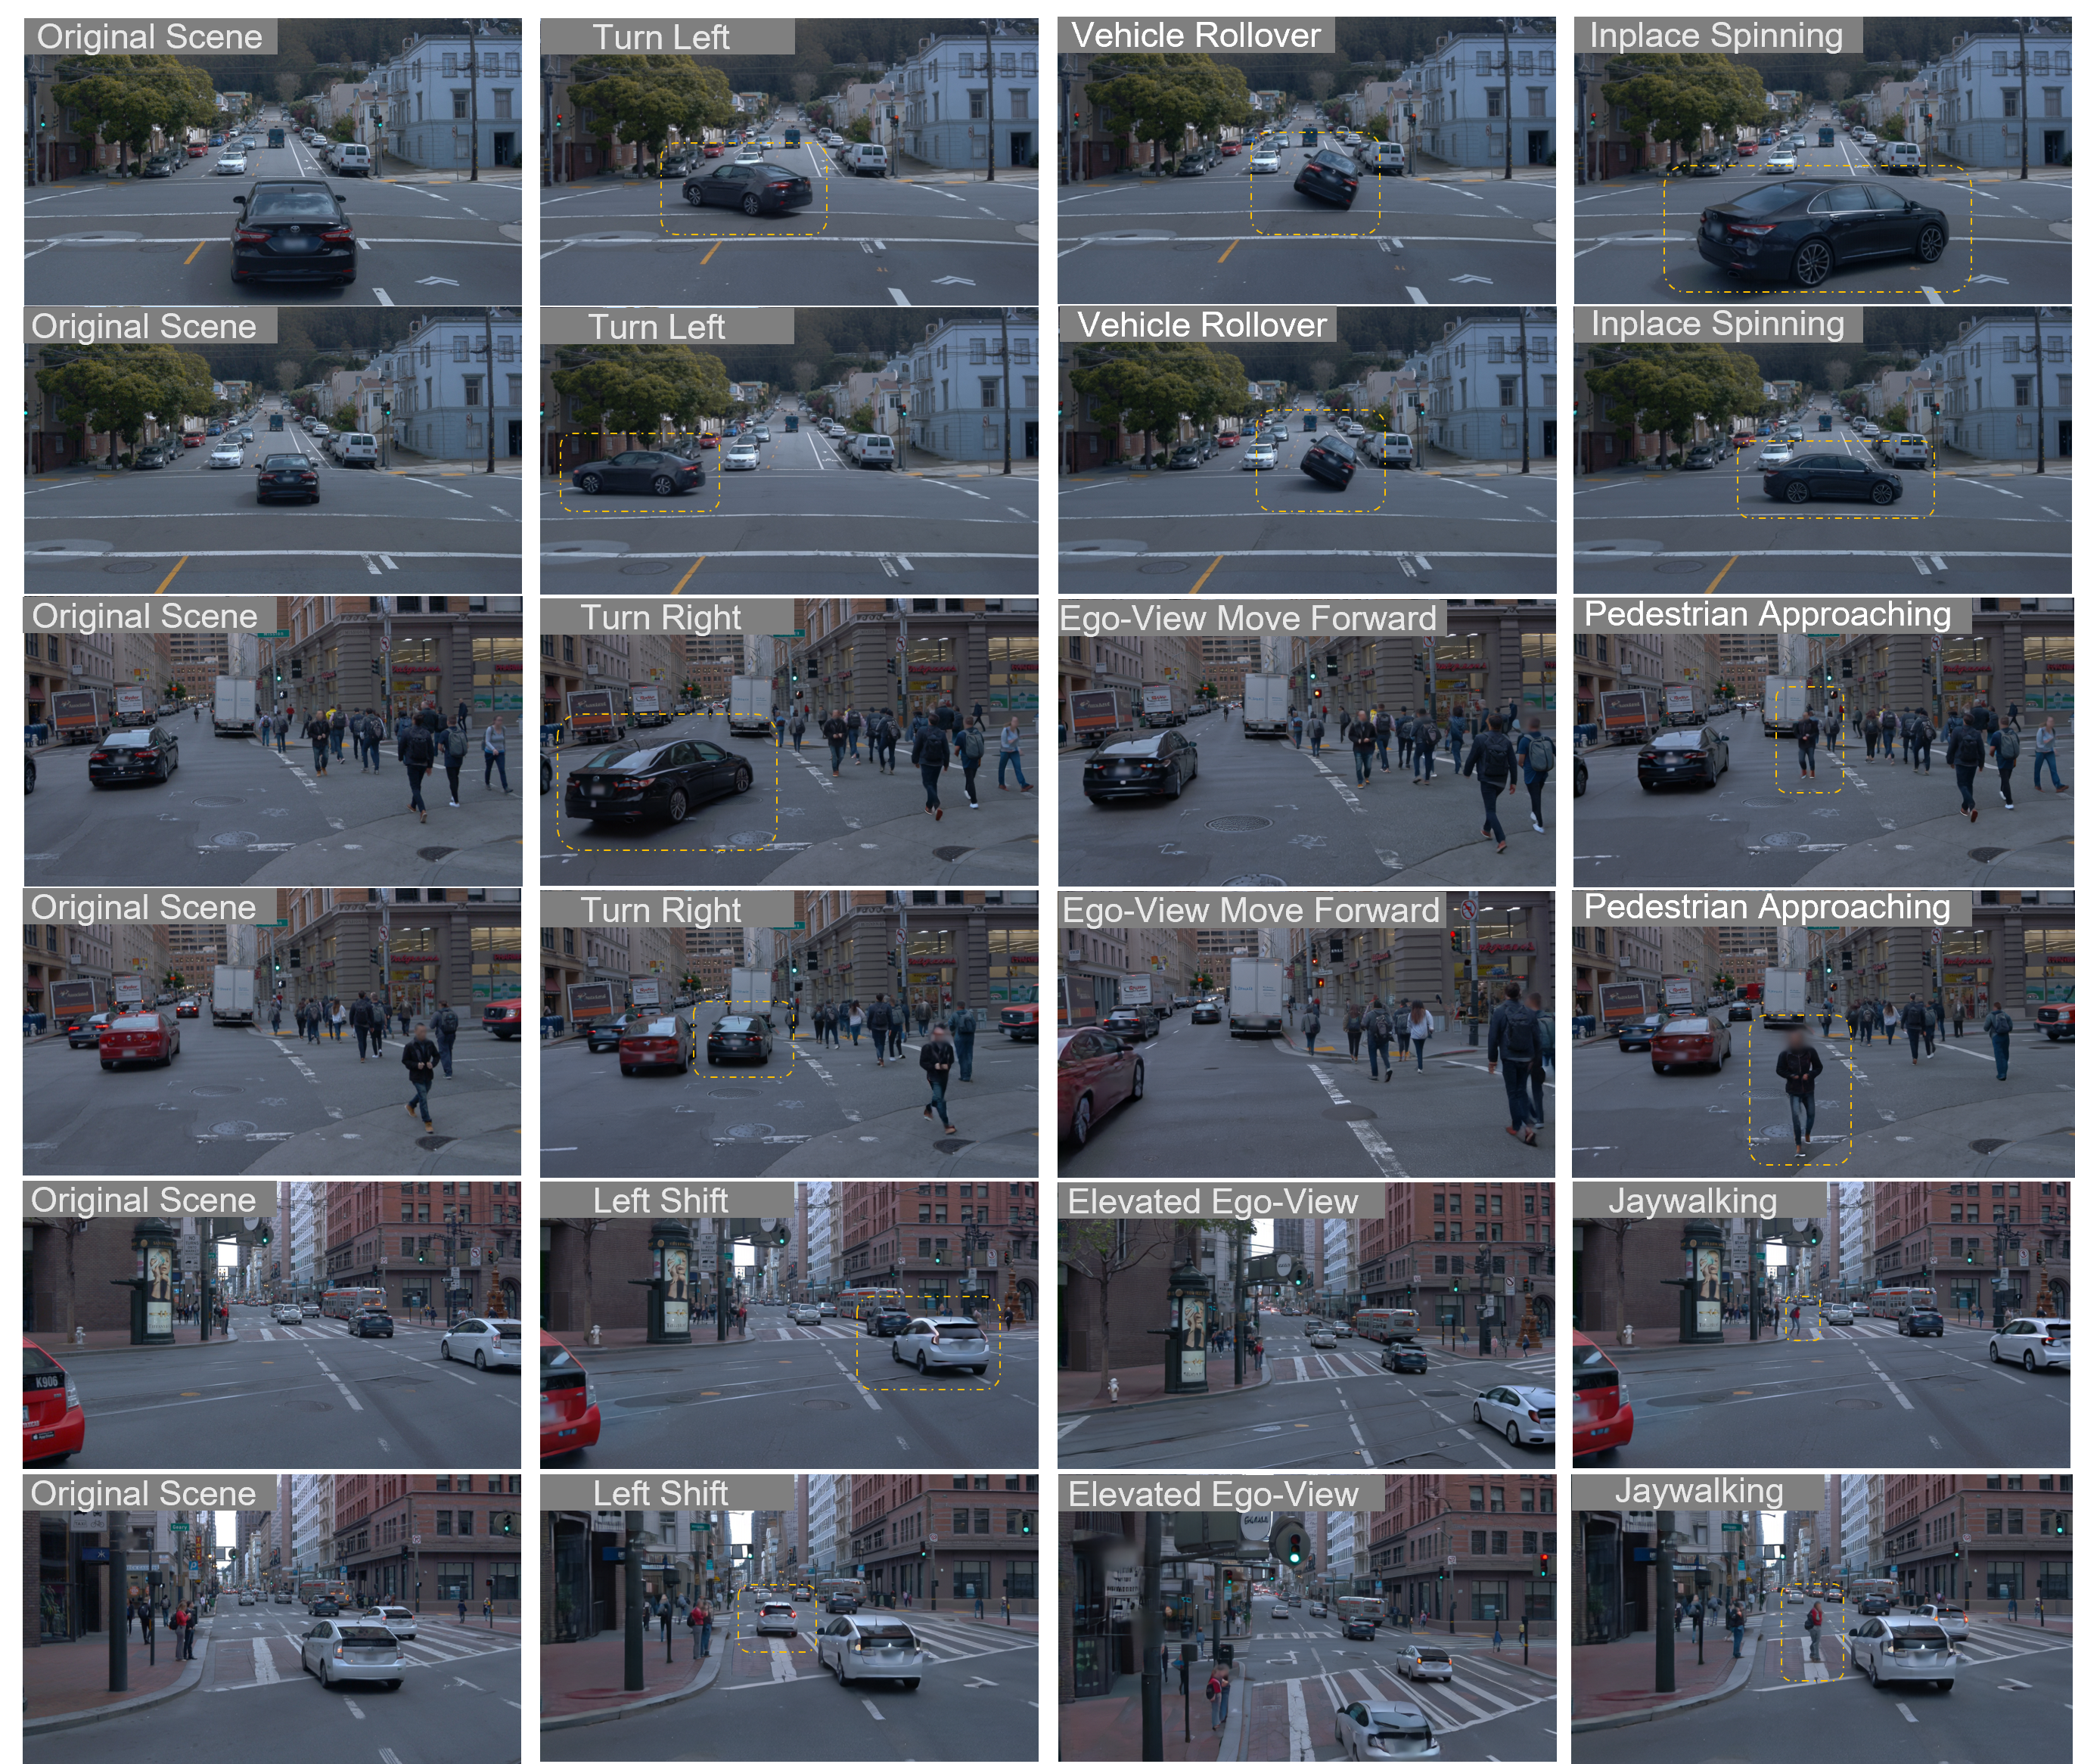
\includegraphics[width=\linewidth]{figures/demo.png}
    \vspace{-0.2in}
    \caption{\textbf{Qualitative demonstrations of ReinDriveGen on OOD safety-critical corner cases.} Every two consecutive rows show two frames from the same scene, with the edit type and edited region annotated in each image.}
    \label{fig:demo}
    \vspace{-0.2in}
\end{figure*}


\subsection{RL-based Post-training}
\label{sec:rl}
The supervised fine-tuning (SFT) stage described in Sec.~\ref{sec:pc_sim} trains the video diffusion model on pairs of
rendered pseudo-images and ground-truth videos, both captured under the original recorded ego-vehicle viewpoints and actor trajectories. At inference time, however, we wish to edit vehicle trajectories (\eg, simulating lead-vehicle collisions, drifting, spinning or other counterfactual maneuvers) or render from novel ego-vehicle viewpoints. In both cases, the rendered pseudo-image conditions deviate significantly from those seen during SFT, exhibiting novel occlusion patterns, unfamiliar vehicle orientations, and untextured completed surfaces, which creates a substantial domain gap.  

% Although the pseudo-view simulation pipeline adopted during SFT (Sec.~\ref{sec:pc_sim}) partially mitigates this gap for novel ego-vehicle viewpoints by simulating edge-aware masking patterns, it is unable to account for the fundamentally different patterns arising from edited actor trajectories, such as vehicles in collision situations, counterfactual paths, or extreme orientations, since such scenarios never occur in the recorded data.

Empirically, we observe that vehicles are the primary source of visual degradation under these out-of-distribution (OOD) conditions, exhibiting distorted geometry, unrealistic textures, and implausible lighting, while static background regions remain largely unaffected. To address this limitation, we propose an RL-based post-training framework that directly optimizes vehicle generation quality under OOD conditions without requiring paired ground-truth supervision.


\subsubsection{Extending DiffusionNFT to Video Generation.}
% We adopt DiffusionNFT~\cite{zheng2025diffusionnft} as our RL post-training framework. DiffusionNFT directly performs policy optimization on the forward diffusion process via the flow matching objective, defining a contrastive improvement direction between implicit positive and negative policies split by reward signals.  Unlike GRPO-style methods~\cite{liu2025flow}, which require storing and backpropagating through full reverse denoising trajectories, DiffusionNFT only requires the final clean outputs and operates in a classifier-free-guidance-free (CFG-free) manner, achieving up to $25\times$ speedup over FlowGRPO~\cite{liu2025flow} as reported in ~\cite{zheng2025diffusionnft}. This efficiency advantage is particularly important for video diffusion RL, where the high dimensionality of spatiotemporal outputs makes both sampling and training substantially more expensive than in the image setting. (说的简短一点)

We adopt DiffusionNFT~\cite{zheng2025diffusionnft} as our RL post-training framework, which achieves significantly faster training than FlowGRPO~\cite{liu2025flow} by performing policy optimization directly on the forward diffusion process in a classifier-free-guidance-free (CFG-free) manner. This efficiency advantage is particularly important for video diffusion RL, where the high dimensionality of spatiotemporal outputs makes both sampling and training substantially more expensive than in the image setting.

We extend DiffusionNFT from image to video generation. Let $\pi_\theta$ denote the video diffusion policy parameterized by $\theta$, and let $\mathbf{c}$ denote a condition consisting of a reference frame and a rendered pseudo-image sequence. We maintain a reference policy $\pi^{\mathrm{old}}$ (updated via EMA) alongside the current policy~$\pi_\theta$. In each iteration, we sample a batch of OOD conditions $\{\mathbf{c}_i\}$.
% , constructed by shifting the ego-vehicle viewpoint laterally or editing vehicle trajectories. 
% (described in Sec.~\ref{sec:reward}XXXX改一下这个，要refer到后面的pairwise的部分)
For each condition, the reference policy generates a group of $N$ candidate videos. A reward model scores each candidate, and the scores are used to optimize the following contrastive objective adapted from DiffusionNFT:
%
\vspace{-0.05in}
\begin{equation}
  \mathcal{L}(\theta)
  = \mathbb{E}_{\mathbf{c},\;
      \pi^{\mathrm{old}}(\mathbf{x}_0|\mathbf{c}),\; t}
    \Big[\,
      r\,\big\lVert
        v_\theta^{+}(\mathbf{x}_t,\mathbf{c},t)-\mathbf{v}
      \big\rVert_2^{2}
      +
      (1-r)\,\big\lVert
        v_\theta^{-}(\mathbf{x}_t,\mathbf{c},t)-\mathbf{v}
      \big\rVert_2^{2}
    \,\Big],
  \label{eq:nft}
\end{equation}
%
where $\mathbf{x}_0$ is a clean generated video sampled from $\pi^{\mathrm{old}}$, $\mathbf{x}_t$ is its noised version at
flow-matching timestep~$t$, $\mathbf{v}$ is the flow-matching velocity target, $r\!\in\![0,1]$ is the reward associated with $\mathbf{x}_0$, and $v_\theta^{+}$, $v_\theta^{-}$ are the implicit positive and negative velocity predictions as defined in~\cite{zheng2025diffusionnft}. Intuitively, for high-reward samples ($r\!\to\!1$) the loss encourages $v_\theta$ to reproduce similar high-quality outputs, while for low-reward samples ($r\!\to\!0$) it steers $v_\theta$ away from low-quality outputs.

%% ------------------------------------------------------------------ %%
\subsubsection{Pairwise Preference Model.}
\label{sec:reward}
A critical component of RL post-training is a reward model that evaluates the quality of vehicles in generated driving videos.
No existing reward model serves this purpose; general-purpose image quality or aesthetics models fail to capture domain-specific artifacts such as distorted vehicle geometry, unrealistic textures, or implausible lighting patterns. We therefore train a dedicated pairwise preference model to evaluate generated vehicle quality.
%,  and build a pairwise reward mechanism on top of it.

\paragraph{Preference data construction.}\quad
To train the pairwise preference model, we need paired data of relatively better and worse vehicle crops. We exploit a key empirical observation: when generating videos with the SFT model, subsampling the pseudo-image conditioning (\ie, providing a rendered pseudo-image every $k$-th frame instead of every frame) progressively degrades the visual quality of vehicles in the generated output.  This provides a natural and controllable mechanism for constructing preference pairs without manual annotation. Concretely, for each scene in the Waymo training dataset, we generate three versions of the output video using the SFT model with pseudo-image conditioning provided at
\emph{(i)}~every frame,
\emph{(ii)}~every 2nd frame, and
\emph{(iii)}~every 4th frame.
Since we focus exclusively on vehicle quality, we apply YOLO26~\cite{sapkota2025yolo26} to detect and crop all vehicle instances from each generated frame.  For a given vehicle instance in a given frame, the crops from different conditioning frequencies form naturally ordered
preference pairs:
(i)$\succ$(ii),\;
(ii)$\succ$(iii),\; and
(i)$\succ$(iii),
all paired on the same vehicle, same frame, and same scene, ensuring that the vehicle quality is the only varying factor.

To further diversify the degradation patterns and improve robustness, we augment both positive and negative samples with motion blur and elastic distortion, where the degradation strength applied to negative samples is always strictly greater than that applied to positive samples. This asymmetric augmentation ensures that the reward model learns to discriminate between relatively better and worse samples even when both exhibit significant artifacts. This property is essential for the early stages of RL training, where the policy generates low-quality outputs and the reward model must still provide a meaningful ranking among candidates to guide optimization. Further details are provided in the supplementary material.


\vspace{-0.2in}
\begin{figure*}[t]
    \centering
    \includegraphics[width=\linewidth]{figures/comparison1.pdf}
    \vspace{-0.2in}
    \caption{Qualitative comparison of novel trajectories in the lane-change scenario.}
    \label{fig:comparison1}
    \vspace{-0.2in}
    %\vspace{-0.2in}
\end{figure*}



\paragraph{Model architecture.}\quad
Given two vehicle crops $I_1$ and $I_2$, we extract their CLS-token representations using a shared DINOv3~\cite{simeoni2025dinov3} ViT-H+ backbone~$f$, yielding $\mathbf{z}_1 = f(I_1)$ and $\mathbf{z}_2 = f(I_2)$ with
$\mathbf{z}_1, \mathbf{z}_2 \in \mathbb{R}^d$.  The two feature vectors are concatenated in both orders and passed through a shared MLP head~$h$ to produce scalar logits $s_{12} = h([\mathbf{z}_1;\,\mathbf{z}_2])$ and
$s_{21} = h([\mathbf{z}_2;\,\mathbf{z}_1])$.  The preference probability is then defined via an antisymmetric formulation:
%
\begin{equation}
  P(I_1 \succ I_2)
  = \sigma\!\Bigl(\frac{s_{12} - s_{21}}{2}\Bigr),
  \label{eq:pref}
\end{equation}
%
where $\sigma$ denotes the sigmoid function.  This design guarantees logical consistency, \ie,
$P(I_1\!\succ\!I_2) = 1 - P(I_2\!\succ\!I_1)$, since $\sigma(-x) = 1 - \sigma(x)$. The pairwise preference model is trained with binary cross-entropy loss on the constructed preference pairs.

\begin{figure*}[t]
    \centering
    \includegraphics[width=\linewidth]{figures/comparison2.pdf}
    \vspace{-0.2in}
    \caption{Qualitative comparison of vehicle trajectory editing. Top two rows: the target vehicle is shifted 6m left and 4m backward. Bottom two rows: the target vehicle is shifted 6m to the right and 1m backward.}
    \label{fig:comparison2}
    \vspace{-0.2in}
    %\vspace{-0.2in}
\end{figure*}



\subsubsection{Pairwise Reward Mechanism.}\quad
Given the trained pairwise preference model, we propose a pairwise reward mechanism to aggregate pairwise comparison outcomes into per-candidate rewards within each group, providing robust training signals for RL-based post-training.

For each OOD condition~$\mathbf{c}$, we generate $N\!=\!16$ candidate videos $\{\mathbf{x}^1,\ldots,\mathbf{x}^N\}$.  Each candidate video is decomposed into individual frames.  We run YOLO26~\cite{sapkota2025yolo26} on the first candidate to detect and localize all vehicles in every frame, yielding a set of bounding boxes.  These bounding boxes are then applied identically to all $N$ candidates, so that exactly the same spatial region is cropped across candidates for fair comparison.  We treat each (frame index, bounding box) tuple as an independent evaluation unit; let $M$ denote the total number of such units across all frames.  For each unit~$m$, we crop the corresponding region from every candidate, producing $N$ crops $\{a_m^1,\ldots,a_m^N\}$.  We then perform all $\binom{N}{2}$ pairwise comparisons using our pairwise preference model (Eq.~\ref{eq:pref}).  For each pair $(a_m^i,a_m^j)$, the model outputs a preference probability $P(a_m^i\!\succ\!a_m^j)$.  The per-unit reward for candidate~$i$ at unit~$m$ is defined as its win rate:
%
\begin{equation}
  R_m^i
  = \frac{1}{N-1}\sum_{j\neq i}
    \mathds{1}\!\Big[P(a_m^i\!\succ\!a_m^j)>\tau\Big],
  \label{eq:winrate}
\end{equation}
%
where $\tau\!=\!0.85$ is a confidence threshold that filters out ambiguous comparisons.  The video-level reward $\hat{R}(\mathbf{x}^i)$ is computed as an area-weighted average of the per-unit win rates across all $M$ units, where each unit is weighted by its bounding-box pixel area so that artifacts on vehicles with larger area are prioritized.  Compared to pointwise scores, pairwise win rates span a wider and more discriminative range and are inherently robust to systematic biases in the reward model.  The resulting $\hat{R}(\mathbf{x}^i)$ is used in place of the pointwise reward~$r$ in the DiffusionNFT loss (Eq.~\ref{eq:nft}), which is seamless as DiffusionNFT only requires a scalar reward per sample. 

With the pairwise reward mechanism in place, we can now perform RL post-training on OOD conditions, such as lead-vehicle collisions, drifting, spinning, and counterfactual trajectories that place vehicles in extreme orientations. In each iteration, the reference policy generates $N\!=\!16$ candidate videos per condition, the pairwise reward mechanism produces a scalar reward~$\hat{R}(\mathbf{x}^i)$ for each candidate, and the policy is updated via the DiffusionNFT objective (Eq.~\ref{eq:nft}) to reinforce high-win-rate generation patterns while suppressing low-quality ones.  This enables the model to progressively improve vehicle quality under OOD conditions without any paired ground-truth supervision.






\section{Experiment}

\subsection{Demonstration of Actor and Viewpoint Manipulation}
Fig.~\ref{fig:demo} demonstrates that our method can manipulate vehicles, pedestrians, and cyclists, including maneuvers outside the training distribution such as in-place spinning, turning, vehicle rollover, and laterally shifted ego-vehicle viewpoints. We encourage the reader to refer to the supplementary material for video results.

% \subsection{Implementation Details}
% \subsubsection{Implementation details of conditional video diffusion model}
% We finetune the video diffusion model on the 1000 scenes of waymo dataset. Each scene consists of 5 views. We only finetune our conditional video diffusion model on the front, front left and front right views. We have trained our video diffusion model for 500 H100 gpu hours based on the VACE1.3B model [XXXX]. We set the batch size to 32 and use the Adam optimizer with constant learning rate 1e-5.

% \subsubsection{Implementation details of RL-Based Post-Training}
% We collect 20 representaive OOD cases such as inplace spinning, turning left or right, vehicle rollover and shifted ego views to train on. We set the number of sample of each condition is 16(这个就是说每次rollout的次数是16，你帮我改成专业的说法).  We set the batch size to 32 and use the Adam optimizer with constant learning rate 1e-5. We keep the same setting of the diffusionNFT training framework such \beta, type of update data collection policy, etc same as the default one(这个也写的专业一点。) We have post-trained the video diffusion model for 400 H100 gpu about 500 steps.

% For the implementation details of the vehicle completion model and the pairwise preference model，please check the supplementory materials. 
\begin{table*}
\centering
\caption{Quantitative comparison in a lane-change scenario where the trajectory gradually shifts 4 m to the left.}
\vspace{-0.1in}
\resizebox{\textwidth}{!}{
\begin{tabular}{l|ccc|ccc|ccc|c}
\toprule
Models &  PVG & \makecell{DD4D w/.\\ PVG} & \makecell{Recon. w/. \\  PVG} & $S^3$Gauss. & \makecell{DD4D w/.\\  $S^3$Gauss.} & \makecell{Recon. w/. \\  $S^3$Gauss.} & Deform.-GS & \makecell{DD4D w/.\\ Deform.-GS} & \makecell{Recon. w/. \\  Deform.-GS} & Ours \\
\midrule
NTA-IoU$\uparrow$ & 0.256 & 0.438  & 0.464 & 0.175 & 0.495 & 0.413 & 0.240 & 0.335 & 0.443 & {\bf 0.549} \\
% LiDAR-only & && \\
NTL-IoU$\uparrow$  & 50.70 & 53.06 & 53.21 & 49.05 & 53.42 & 51.62 & 51.62 & 52.93 & 53.78 & {\bf 56.13}  \\
FID$\downarrow$  & 105.29 & 71.52 & 74.32 & 124.90 & 66.93 & 123.61 & 92.24 & 77.32 & 76.24 & {\bf 51.99}\\

\bottomrule
\end{tabular}}

\label{tab:table_comparison1}
\end{table*}
\vspace{-0.3in}


\subsection{Implementation Details}

\subsubsection{Conditional Video Diffusion Model.}
We fine-tune the video diffusion model on 1{,}000 scenes from the Waymo dataset~\cite{Sun_2020_CVPR}. Each scene comprises five camera views; we use only the front, front-left, and front-right views for training. Starting from the VACE-1.3B model~\cite{jiang2025vace}, we fine-tune for approximately 500 H100 GPU hours with a batch size of 32, using the Adam optimizer with a constant learning rate of $1\!\times\!10^{-5}$.

\subsubsection{RL-Based Post-Training.}
We curate 20 representative OOD conditions covering in-place spinning, left/right turning, vehicle rollover, and laterally shifted ego-vehicle viewpoints. For each condition, we generate a group of $N=16$ candidate videos per rollout for policy optimization. To ensure training stability, we adopt LoRA for RL-based fine-tuning rather than updating full model weights. We use the Adam optimizer with a constant learning rate of $1\!\times\!10^{-5}$. All other hyperparameters of the DiffusionNFT framework, including $\beta$ and the data collection policy update strategy, follow the default settings in~\cite{zheng2025diffusionnft}. Post-training takes approximately 400 H100 GPU hours over 500 optimization steps.

For implementation details of the vehicle completion model and the pairwise preference model, please refer to the supplementary material.

\begin{figure}
    \centering
    \includegraphics[width=\linewidth]{figures/ablation_completion.pdf}
    \vspace{-0.2in}
    \caption{\textbf{Ablation study on vehicle completion.} Vehicle completion fills in unobserved surfaces in the pseudo-images, effectively eliminating vehicle distortion and texture artifacts in the diffusion outputs.}
    \label{fig:ablation_completion}
    %\vspace{-0.2in}
\end{figure}

\vspace{-0.2in}


\subsection{Comparison}
We compare our method against existing approaches under two evaluation settings: novel ego-vehicle trajectory and vehicle trajectory editing.

\subsubsection{Novel Ego-Vehicle Trajectory.}
We evaluate on the off-trajectory benchmark proposed by DriveDreamer4D~\cite{zhao2024drive}, which introduces Novel Trajectory Agent IoU (NTA-IoU) and Novel Trajectory Lane IoU (NTL-IoU) to measure spatial consistency of vehicles and lane boundaries under novel viewpoints. To simulate a realistic lane-change scenario, we apply a lateral shift of 0.1\,m per frame over 40 frames, yielding a cumulative lateral shift of 4\,m. We compare with PVG~\cite{chen2026periodic}, DriveDreamer4D~\cite{zhao2024drive}, ReconDreamer~\cite{ni2025recondreamer}, S3Gaussian~\cite{huang2024s3gaussian}, and Deformable-GS~\cite{yang2023deformable3dgs}. We additionally report FID between original-trajectory and novel-trajectory images to evaluate photorealism. As shown in Tab.~\ref{tab:table_comparison1}, our method achieves the best performance across all metrics. The qualitative comparison in Fig.~\ref{fig:comparison1} is consistent with the quantitative results: our method produces the most photorealistic outputs. Since FreeVS~\cite{wang2024freevs} only generates partial novel views, we include it in qualitative comparisons only.




% \begin{table}[ht]
%   \centering
% \caption{Quantitative comparison in the Vehicle Trajectory Editing scenario.}
%   % 调整列间距，如果觉得太宽可以改小，默认约 6pt
%   \setlength{\textwidth}{3pt} 
%   \begin{tabular}{l|c|c|c|c}
%     \toprule
%     Method & Motion smoothness$\uparrow$ & Background consistency$\uparrow$ & Image quality$\uparrow$ & FID$\downarrow$ \\

%     \midrule
    
%     Street Gauss. & 0.981111 & 0.930975 & 0.639775 & 84.7970 \\
%     StreetCrafter    & {\bf 0.981715} & 0.906872 & 0.650856 & 83.6278 \\
%     Ours             & 0.977355 & {\bf 0.939697} & {\bf 0.692809} & {\bf 80.6267} \\
%     \bottomrule
%   \label{tab:quantitative_comparison2}
%   \end{tabular}
% \end{table}



\begin{table}[t]
  \centering
  \caption{Quantitative comparison on the vehicle trajectory editing scenario with a 5m lateral shift.}
  \vspace{-0.1in}
  \label{tab:quantitative_comparison2}
  \setlength{\textwidth}{3pt} 

  % 保留竖线
  \begin{tabular}{l|c|c|c|c}
    \hline  % 用双横线模拟 toprule
    Method & Motion smoothness$\uparrow$ & Background consistency$\uparrow$ & Image quality$\uparrow$ & FID$\downarrow$ \\
    \hline % 用 hline 模拟 midrule
    Street Gauss. & 0.981111 & 0.930975 & 0.639775 & 84.7970 \\
    StreetCrafter & {\bf 0.981715} & 0.906872 & 0.650856 & 83.6278 \\
    Ours          & 0.977355 & {\bf 0.939697} & {\bf 0.692809} & {\bf 80.6267} \\
    \hline % 用 hline 模拟 bottomrule
  \end{tabular}
  \vspace{-0.2in}
\end{table}






\begin{figure}
    \centering
    
\includegraphics[width=\linewidth]{figures/ablation.pdf}
    \vspace{-0.2in}
    \caption{\textbf{Ablation study on RL-based post-training.} From top to bottom: doubled vehicle speed, in-place spinning, and vehicle rollover. As the RL training step increases, the generated vehicles exhibit progressively better geometry, texture fidelity, and lighting plausibility.}
    \label{fig:ablation}
    %\vspace{-0.2in}
    \vspace{-0.2in}
\end{figure}


\subsubsection{Vehicle Trajectory Editing.}
Since several recent methods, including DriveDreamer4D~\cite{zhao2024drive}, ReconDreamer~\cite{ni2025recondreamer}, and FreeSim~\cite{fan2025freesim}, have not released their source code, we compare with Street Gaussians~\cite{yan2024street} and StreetCrafter~\cite{yan2025streetcrafter} on this setting. We keep the ego-vehicle trajectory fixed and manually edit a target vehicle's trajectory to evaluate each method's ability to handle modified scenes. The qualitative comparison is shown in Fig.~\ref{fig:comparison2}. Street Gaussians and StreetCrafter fail to synthesize plausible content in regions that are unobserved in the original recorded views and produce incorrect lighting on the edited vehicles. In contrast, our method successfully generates realistic content for invisible regions from the recorded views and produces photorealistic lighting. For quantitative evaluation, we adopt three metrics from VBench~\cite{huang2023vbench}, namely image quality, background consistency, and motion smoothness, and evaluate on the 5 scenes released by StreetCrafter with a 5\,m lateral vehicle shift. As shown in Tab.~\ref{tab:quantitative_comparison2}, our method achieves the best performance in FID, image quality, and background consistency.




% \subsubsection{Comparison on the off-trajectory view}
% We test our methods on the off-trajectory evaluation benchmarks proposed by the drivedreamer4d [XXX], in which the metrics Novel trajectory Agent IoU (NTA-IoU) and Novel Trajectory Lane IoU (NTL-IoU), to evaluate spatial consistency of vehicles and lane boundaries in novel views. To better simulate realistic driving scenarios, we evaluate methods on a lane change trajectory with a lateral shift of 0.1 meters per frame over 40 frames, producing a total lateral shift of 4m. We compare our methods with PVG[XXX], DriveDreamer4D[XXX],  ReconDreamer[XXX], S3Gaussian[XXX] and Deformable-GS[XXX]. We also report the FID between original and novel trajectory images to evaluate photorealism. Table[XXXX] show that our method achieve the better among all methods. And we also provide the qualitative comparison as shown the Fig [XXX], which also align with the numerical results. We method achieve the most photorealistic results.  


% \subsubsection{Comparison on (编辑过车辆轨迹的场景。)}
% Since lots of methods do not release their codes such as DriveDreamer4D[XXXX], ReconDreamer[XXX], Freesim[XXX], etc, We compare our method with Street Gaussians[XXX] and Streetcrafter[XXX]. We manually change a vehicle's trajectory and compare the results. The qualitative comparison is shown in the figure[XXX]. From the figure, we can know that the Street Gaussians and Streetcrafter fail to sythesize realistic view on the region that is invisble to the recorded views and also fail to generate realistic lighting of the edited cars. Whereas, ours method manage to generated the invisble regions to the recorded views and also generate correct lighting of the edited cars. We evaluate street Gaussians, streetcrafter and our method in terms of metrics of Vbench [XXX]. We evaluate on the 5 scenes released by the streetcrafter with 5 meter left or right car shift based on the 具体的场景。Table[XXX] show the results, our method achieves the best in term of Fid, Image quality  and background consistency. 


\begin{figure*}
    \centering
    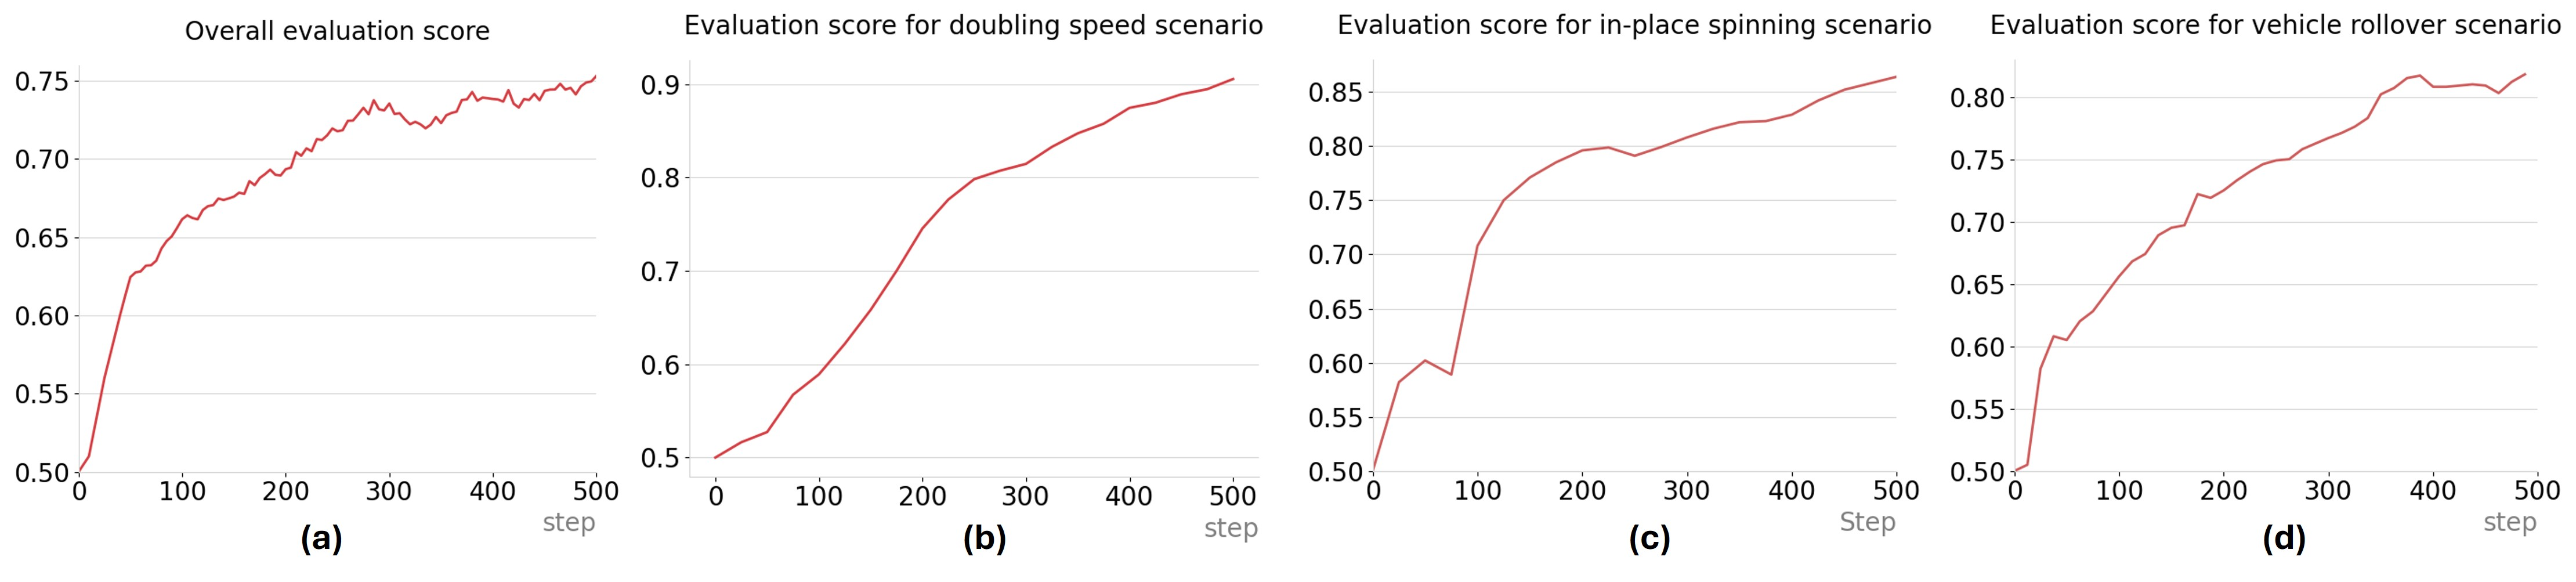
\includegraphics[width=\linewidth]{figures/curve_reward.jpg}
    \vspace{-0.3in}
    \caption{\textbf{Evaluation score curves during RL training.} (a) Overall evaluation score averaged across all OOD conditions. (b)--(d) Per-scenario scores for doubling speed, in-place spinning, and vehicle rollover, respectively.}
    \label{fig:curve_reward}
    \vspace{-0.3in}
    %\vspace{-0.2in}
\end{figure*}


% \subsection{Ablation study}
% In this section we 验证一下这个vechile completion和这个post training 到底有没有用（变成学术的说法）

% \subsubsection{Ablation study on the vehicle completion}
% To verify the effectiveness of the vehicle completion, we test the performance on an edit car trajectory的情景,这个情景会reposition 这个vechile，把原轨迹不可见的区域露出，这样更可以体现vechile completion的重要性。Fig[XXX]展示了pseudo-image w/ and w/o vechile completion, and corresponding video diffusion results. From the visual result, we can know that the vechile completion 确保了vechile的几何一致性和表面纹理的正确性，由没有vechile completion生成的有明显的vechile distortion和表面纹理的artifacts.

% \subsubsection{Ablation study on the RL-Based Post-Training}
% Since we adopt the pairwise reward model, 不是同一个sample rollout里面的无法直接比较。所以，在每跑完5个step之后，我们进行一次evaluation。我们是这么设计evaluation的：在把seed都设置成0，这样排除randomness的影响。然后在相同的condition的条件下，没有rl的video diffusion和rl之后的video diffusion model各自生成一个视频。在这两个视频之间，我们可以算一个evaluation score来衡量rl之后的diffusion model是不是有进步。这个算法和pairwise reward mechanism类似，相当于，N=2,然后照样得到那个tuple， 因为这里只有两个video，所以那个R^-_m可以直接定义成 P（a^i_m > a^j_m）的数值，然后同样的计算area-weighted average of the per unit across all M units。这样我们就得到了一个衡量这两个视频的指标，然后在全部的condition上都算一遍，算一个平均。这样我们的就得到了一个可以判断video diffusion是否有进步的指标。这个RL training 的指标展示在figureXXX （a).

% 在step 0的时候，这个 P（a^i_m > a^j_m）恒等于0.5. rea-weighted average of the per unit across all M units也等于0. 所以这个evaluation score 是从0.5开始上升的。）. 同时我们还展示了3个例子，在rl 过程中，不同step时候的visual result()，同样的，在生成这个visual results的时候，set the seed=0,为了可以公平的对比在不同rl training step时候的结果。这三个例子从上往下分别是，1. 车速变成原来的两倍 2. vehicle inplace spinning, 3. vehicle rollover. 从这个figure里面，我们可以观察到，这个video diffusion model在OOD的条件下，生成的结果逐渐变好的过程,展示了这个rl post training的作用。 这三个例子的自己的evaluation的score也展示在figureXXX （b), (c), (d), repesctively. 



\subsection{Ablation Studies}
We conduct ablation studies to validate the effectiveness of two key components of our framework: vehicle point cloud completion (Sec.~\ref{sec:pc_sim}) and RL-based post-training (Sec.~\ref{sec:rl}).

\subsubsection{Effect of Vehicle Completion.}
To isolate the contribution of vehicle completion, we evaluate on a vehicle trajectory editing scenario where a target vehicle is repositioned along a modified path, exposing surfaces that are unobserved in the original recording. This setting is specifically chosen because repositioned vehicles are viewed from novel angles, making geometric completeness critical. Fig.~\ref{fig:ablation_completion} presents the rendered pseudo-images with and without vehicle completion, along with the corresponding video diffusion outputs. With vehicle completion, the pseudo-images provide geometrically complete vehicle silhouettes, enabling the diffusion model to produce vehicles with consistent geometry and plausible textures. Without it, large holes on occluded surfaces lead to noticeable vehicle distortion and severe texture artifacts, confirming that vehicle completion is essential for high-quality generation under trajectory edits.

% \subsubsection{Effect of RL-Based Post-Training.}
% \label{sec:ablation_rl}
% Since VehiclePrefNet is a pairwise preference model, samples from different rollouts cannot be directly compared via absolute scores.（这里说的不对，我的意思是，在每次rollout中得到的那个reward，也就是从pairwise reward mechanism得到的这个reward，不能在不同的sample里面比较，你明白我的意思吗，这个reward只在计算他的那个group里有效，出了那个group就无效了。） We therefore design a dedicated evaluation method that is executed every 5 training steps. Specifically, we fix the random seed to 0 to eliminate stochasticity, and for each OOD condition~$\mathbf{c}$, we generate one video from the SFT baseline $\pi_{\mathrm{sft}}$ and one from the current RL-trained model $\pi_{\theta_k}$ at step~$k$, both under identical conditions and the same seed. We then apply the same vehicle detection and cropping procedure described in Sec.~\ref{sec:reward} to obtain $M$ evaluation units. For each unit~$m$, we compute the pairwise preference probability $P(a_m^{\mathrm{rl}}\!\succ\!a_m^{\mathrm{sft}})$ using VehiclePrefNet. The per-condition （这个per-condtion，会不会让作者有歧义，这里其实有两个evaluation score，一个是在全部的condition上算average，一个是只看一个condition的，怎么才能说的清楚呢？）evaluation score is defined as the area-weighted average of these preference probabilities across all $M$ units:
% %
% \begin{equation}
%   E(\mathbf{c})
%   = \frac{\sum_{m=1}^{M} w_m \cdot P(a_m^{\mathrm{rl}}\!\succ\!a_m^{\mathrm{sft}})}
%          {\sum_{m=1}^{M} w_m},
%   \label{eq:eval}
% \end{equation}
% %
% where $w_m$ is the bounding-box pixel area of unit~$m$. The overall evaluation score is obtained by averaging $E(\mathbf{c})$ across all evaluation conditions. At step~0, the RL model is identical to the SFT baseline, so both models produce the same video under the same seed, yielding $P(a_m^{\mathrm{rl}}\!\succ\!a_m^{\mathrm{sft}})=0.5$ for all units and hence $E=0.5$. A score rising above 0.5 indicates that the RL-trained model generates higher-quality vehicles than the SFT baseline.

% Figure~\ref{XXX}\,(a) shows the overall evaluation score over the course of RL training, demonstrating a steady improvement as training progresses. We additionally present three representative OOD scenarios in Figure~\ref{XXX}, with all visualizations generated using a fixed seed of 0 for fair comparison across different training steps. From top to bottom, the three scenarios are: (1)~doubling the original vehicle speed, (2)~in-place vehicle spinning, and (3)~vehicle rollover. The visual results clearly show a progressive refinement in vehicle geometry, texture fidelity, and lighting plausibility as RL training proceeds, confirming that the post-training framework effectively improves generation quality under OOD conditions. The per-scenario evaluation scores are reported in Figure~\ref{XXX}\,(b),\,(c), and\,(d), respectively, all exhibiting consistent upward trends that corroborate the qualitative observations.


\subsubsection{Effect of RL-Based Post-Training.}
\label{sec:ablation_rl}
Since the pairwise reward mechanism (Eq.~\ref{eq:winrate}) computes win rates within each group of $N$ candidates sampled for a given condition, the resulting rewards reflect only relative quality rankings within that group. They are not comparable across different groups. We therefore design a dedicated evaluation method that is executed every 5 training steps. Specifically, we fix the random seed to 0 to eliminate stochasticity, and for each OOD condition~$\mathbf{c}$, we generate one video from the SFT baseline $\pi_{\mathrm{sft}}$ and one from the current RL-trained model $\pi_{\theta_k}$ at step~$k$, both under identical conditions and the same seed. We then apply the same vehicle detection and cropping procedure described in Sec.~\ref{sec:reward} to obtain $M$ evaluation units. For each unit~$m$, we compute the pairwise preference probability $P(a_m^{\mathrm{rl}}\!\succ\!a_m^{\mathrm{sft}})$ using our pairwise preference model . The evaluation score for a single condition is defined as the area-weighted average of these preference probabilities across all $M$ units:
%
\begin{equation}
  E(\mathbf{c})
  = \frac{\sum_{m=1}^{M} w_m \cdot P(a_m^{\mathrm{rl}}\!\succ\!a_m^{\mathrm{sft}})}
         {\sum_{m=1}^{M} w_m},
  \label{eq:eval}
\end{equation}
%
where $w_m$ is the bounding-box pixel area of unit~$m$. The overall evaluation score is then obtained by averaging $E(\mathbf{c})$ across all evaluation conditions. At step~0, the RL model is identical to the SFT baseline, so both models produce the same video, yielding $P(a_m^{\mathrm{rl}}\!\succ\!a_m^{\mathrm{sft}})=0.5$ for all units and hence an overall score of $0.5$. A score rising above $0.5$ indicates that the RL-trained model generates higher-quality vehicles than the SFT baseline.

Fig.~\ref{fig:curve_reward}\,(a) shows the overall evaluation score over the course of RL training, demonstrating a steady improvement as training progresses. We additionally present three representative OOD scenarios in Fig.~\ref{fig:ablation}, with all visualizations generated using a fixed seed of 0 for fair comparison across different training steps. From top to bottom, the three scenarios are: (1)~doubling the original vehicle speed, (2)~in-place vehicle spinning, and (3)~vehicle rollover. The visual results clearly show a progressive refinement in vehicle geometry, texture fidelity, and lighting plausibility as RL training proceeds, confirming that the post-training framework effectively improves generation quality under OOD conditions. The per-scenario evaluation scores are reported in Fig.~\ref{fig:curve_reward}\,(b),\,(c), and\,(d), respectively, all exhibiting consistent upward trends that corroborate the qualitative observations.



\subsection{Limitations and Conclusion}
\label{sec:conclusion}


We have presented ReinDriveGen, a unified framework for photorealistic and freely editable driving scene simulation that combines explicit 3D point cloud editing with diffusion-based video synthesis. A vehicle completion module enables free-form manipulation of vehicle trajectories without geometric artifacts, and an RL-based post-training strategy with a pairwise reward mechanism substantially improves vehicle quality under out-of-distribution scenarios. Currently, our method is constrained by GPU memory to generating 49-frame clips, with each clip taking approximately one minute, which does not yet support real-time applications.

More broadly, our work demonstrates that RL-based post-training can effectively improve diffusion model performance beyond the coverage of supervised training data. In autonomous driving, safety-critical corner cases, such as in-place spinning and vehicle rollover, are inherently rare, making the resulting distribution gap a fundamental challenge rather than a data collection problem. The proposed approach offers a principled solution to this challenge, and we believe the same paradigm can be extended to other domains where training data cannot fully cover the space of desired test-time conditions.



% ---- Bibliography ----
%
% BibTeX users should specify bibliography style 'splncs04'.
% References will then be sorted and formatted in the correct style.
\bibliographystyle{splncs04}
\bibliography{main}

\newpage
\appendix

\section{Details of Point Completion Model}
We fine-tune a pre-trained AdaPoinTr~\cite{yu2021pointr} model on the car category of Projected ShapeNet-55~\cite{chang2015shapenet} for 600 epochs. To bridge the sim-to-real gap with real-world KITTI LiDAR data, we simulate single-sided sensor visibility using 16 viewpoints per CAD model and inject synthetic noise. The model takes 2,048 sampled points as input and predicts 8,192 complete points. During training, we apply multi-view random sampling and X/Z-axis mirroring for data augmentation. We optimize the standard AdaPoinTr architecture (6-layer encoder, 8-layer decoder) using AdamW with a batch size of 32, an initial learning rate of \(1 \times 10^{-4}\), and a weight decay of \(5 \times 10^{-4}\).

\section{Details of Pairwise Preference Model} 
To prevent the preference model from trivially relying on low-level image sharpness, we introduce an asymmetric adversarial augmentation strategy. Specifically, we degrade high-quality images using structural-preserving perturbations (e.g., motion blur, ghosting, Gaussian blur, and elastic transformations), while artificially sharpening low-quality images via unsharp masking alongside structural distortions. With the DINOv3 backbone frozen, we train the preference head for 15 epochs using the AdamW optimizer. We set the batch size to 32, the initial learning rate to \(1 \times 10^{-5}\), and the weight decay to \(0.05\). The learning rate is decayed following a cosine schedule with a \(10\%\) warmup ratio. The network is optimized using a Binary Cross-Entropy (BCE) loss applied to the symmetric difference of the pairwise logits.


\begin{figure}
    \centering
    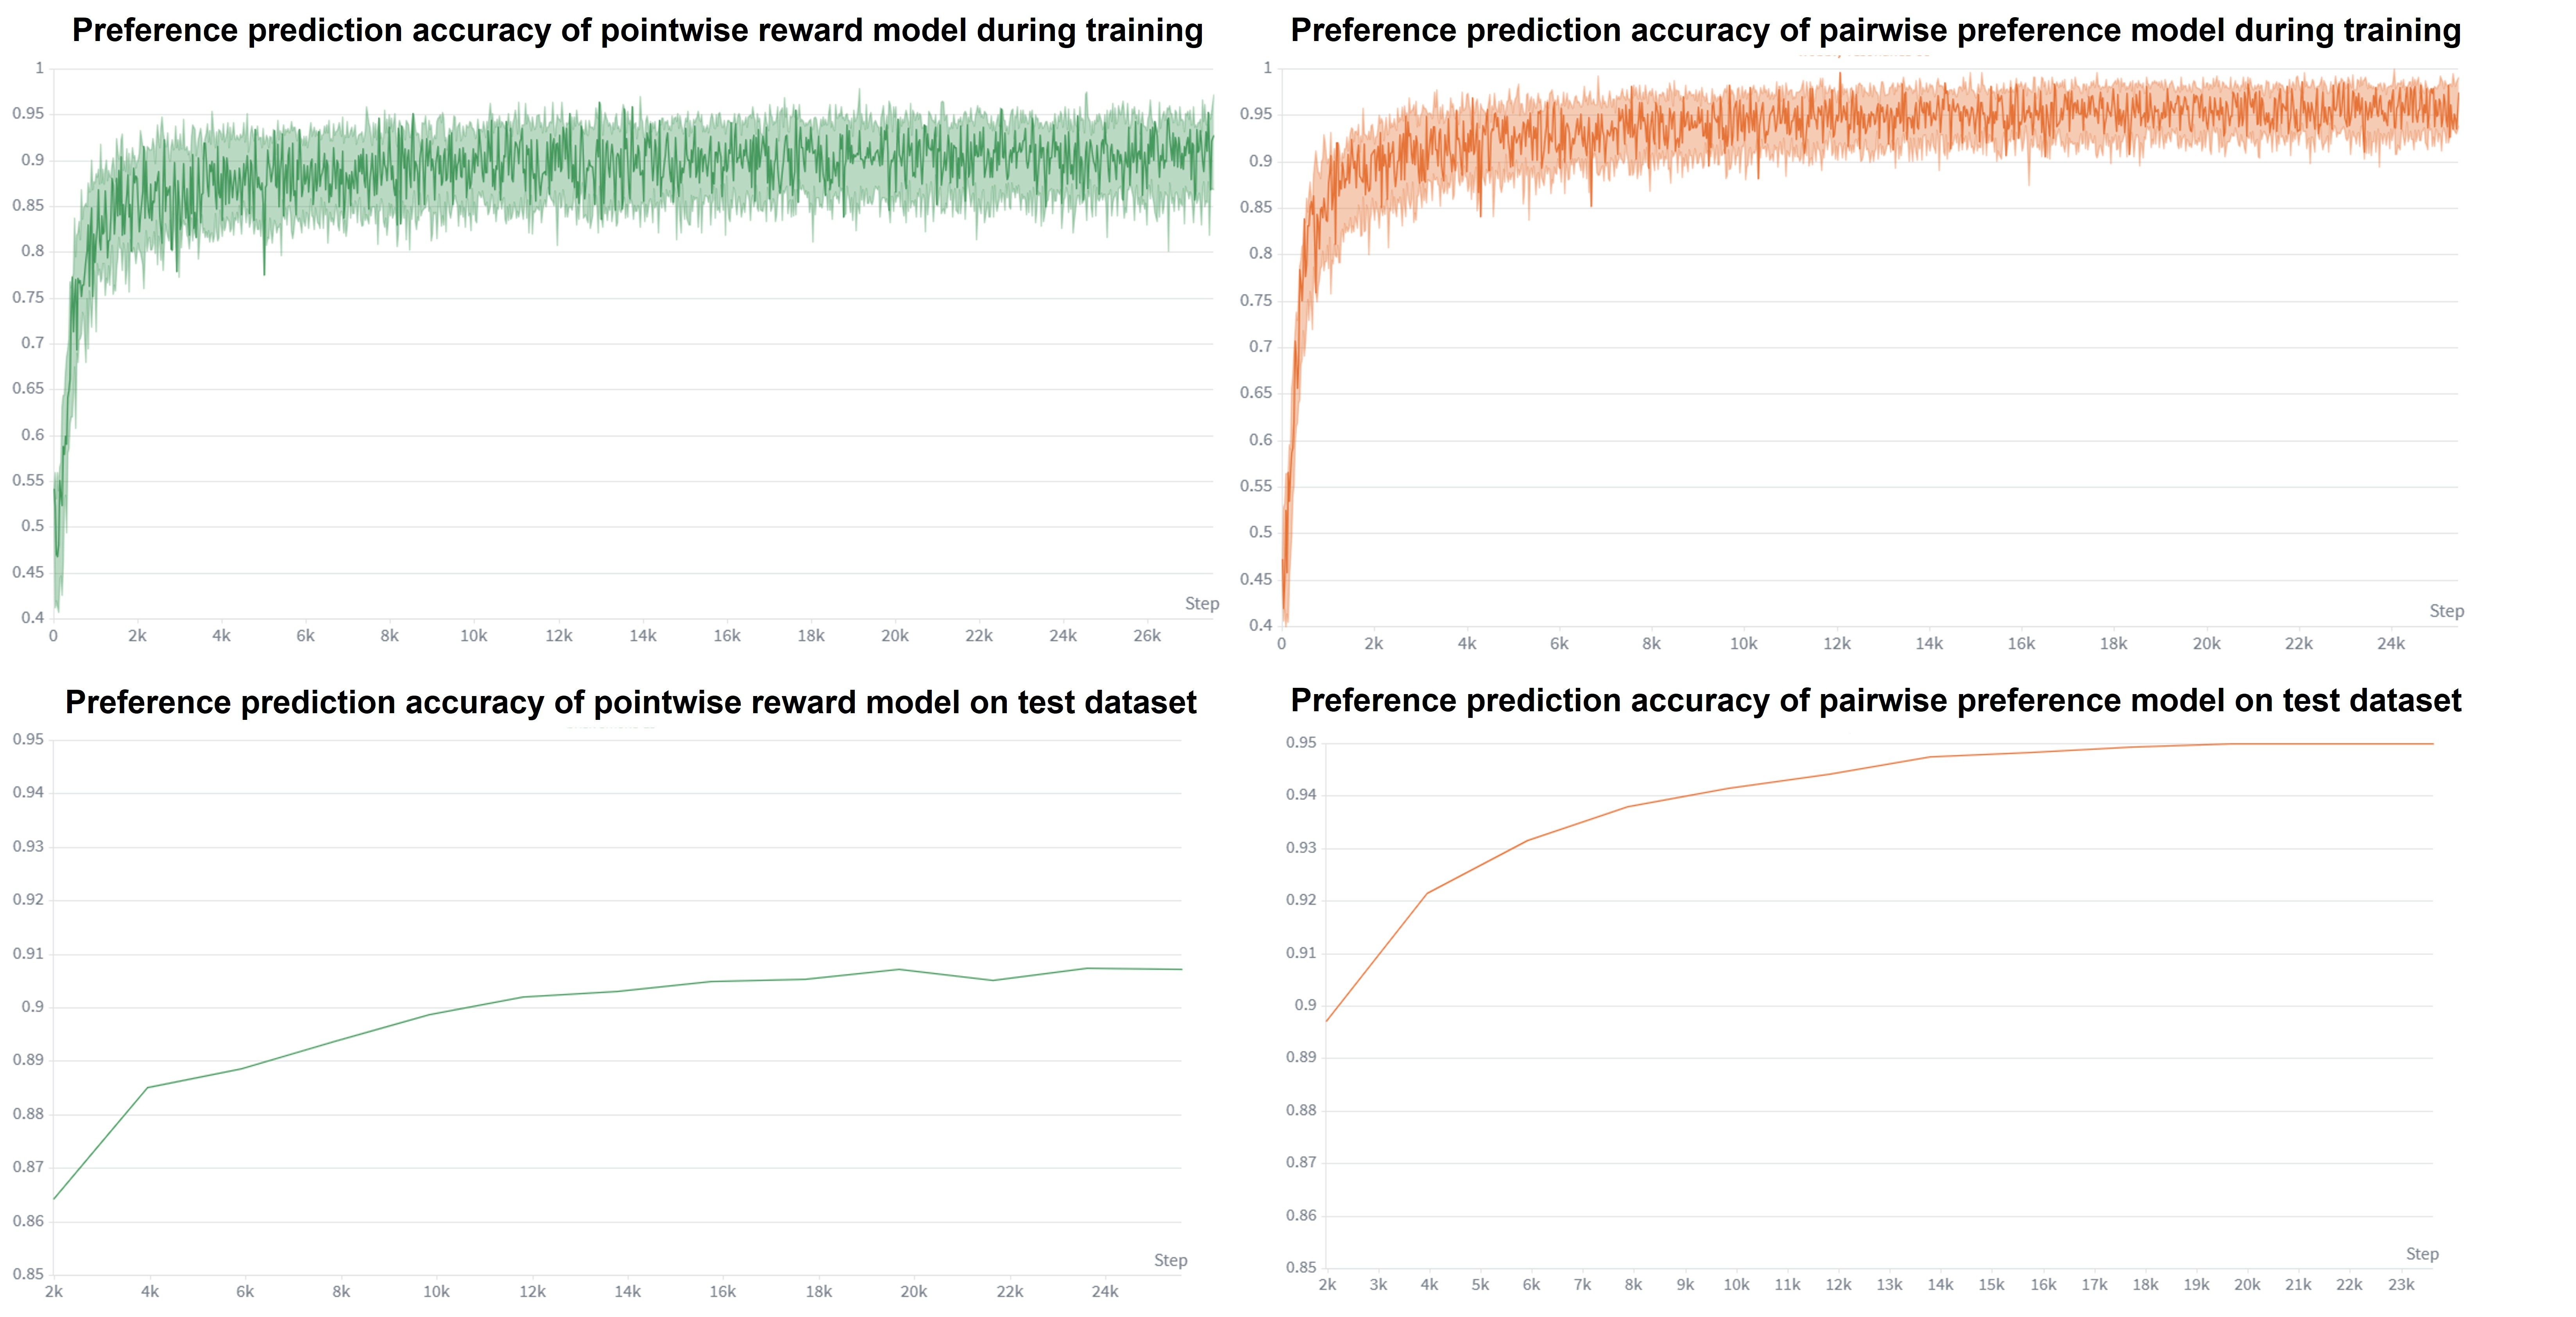
\includegraphics[width=\linewidth]{figures/pointwise_pairwise_curve.jpg}
    \vspace{-0.2in}
    \caption{Preference prediction accuracy of the pointwise reward model (green) and the pairwise preference model (orange) during training (top) and on the test set (bottom). The pairwise model achieves higher test-set accuracy (95\% vs.\ 91\%) with more stable training dynamics, demonstrating that jointly contrasting two samples within a shared forward pass yields more robust preference judgments than independent pointwise scoring.}
    \label{fig:pointwise_pairwise_curve}
    %\vspace{-0.2in}
    \vspace{-0.2in}
\end{figure}


\section{Ablation study on the Pairwise Reward model and the Pointwise Reward model}

\noindent\textbf{Pairwise vs.\ Pointwise Reward Model.}
A core design choice in our RL-based post-training is the use of a pairwise preference model (Sec.3.2) rather than a conventional pointwise reward model. To validate this choice, we train a pointwise baseline and compare both models in terms of preference prediction accuracy and downstream RL post-training quality.

\subsection{Pointwise reward model.}
The pointwise baseline shares the same frozen DINOv3~\cite{simeoni2025dinov3} ViT-H+ backbone as our pairwise model to extract CLS-token representations. Instead of jointly comparing two crops through the antisymmetric formulation, it attaches an independent MLP head $g$ that maps each CLS-token to a scalar quality score in $[0,1]$. The head architecture is: $\mathrm{Linear}(d, 1024) \!\to\! \mathrm{LN} \!\to\! \mathrm{GELU} \!\to\! \mathrm{Dropout}(0.1) \!\to\! \mathrm{Linear}(1024, 512) \!\to\! \mathrm{LN} \!\to\! \mathrm{GELU} \!\to\! \mathrm{Linear}(512, 1) \!\to\! \mathrm{Sigmoid}$, where $d$ is the backbone hidden dimension and $\mathrm{LN}$ denotes LayerNorm. Given two vehicle crops $I_1$ and $I_2$, the model independently computes scalar scores $r_1 = g(f(I_1))$ and $r_2 = g(f(I_2))$, and the preference probability under the Bradley-Terry framework is:
\begin{equation}
    P(I_1 \succ I_2) = \sigma(r_1 - r_2),
    \label{eq:bt}
\end{equation}
where $\sigma$ is the sigmoid function. Crucially, each image receives an absolute score in isolation, and the preference is determined solely by the difference of two independently computed scalars. The model is trained by maximizing the Bradley-Terry log-likelihood: $\mathcal{L}_{\mathrm{pt}} = -\log \sigma(r_{\mathrm{pos}} - r_{\mathrm{neg}})$.


\subsection{Preference accuracy comparison.}
Fig.~\ref{fig:pointwise_pairwise_curve} presents the preference prediction accuracy of both models on the training and test sets. The pairwise model consistently achieves higher test-set accuracy with more stable training dynamics, confirming that directly contrasting two samples within a shared forward pass yields more robust preference judgments than assigning absolute scores independently.

\begin{figure}
    \centering
    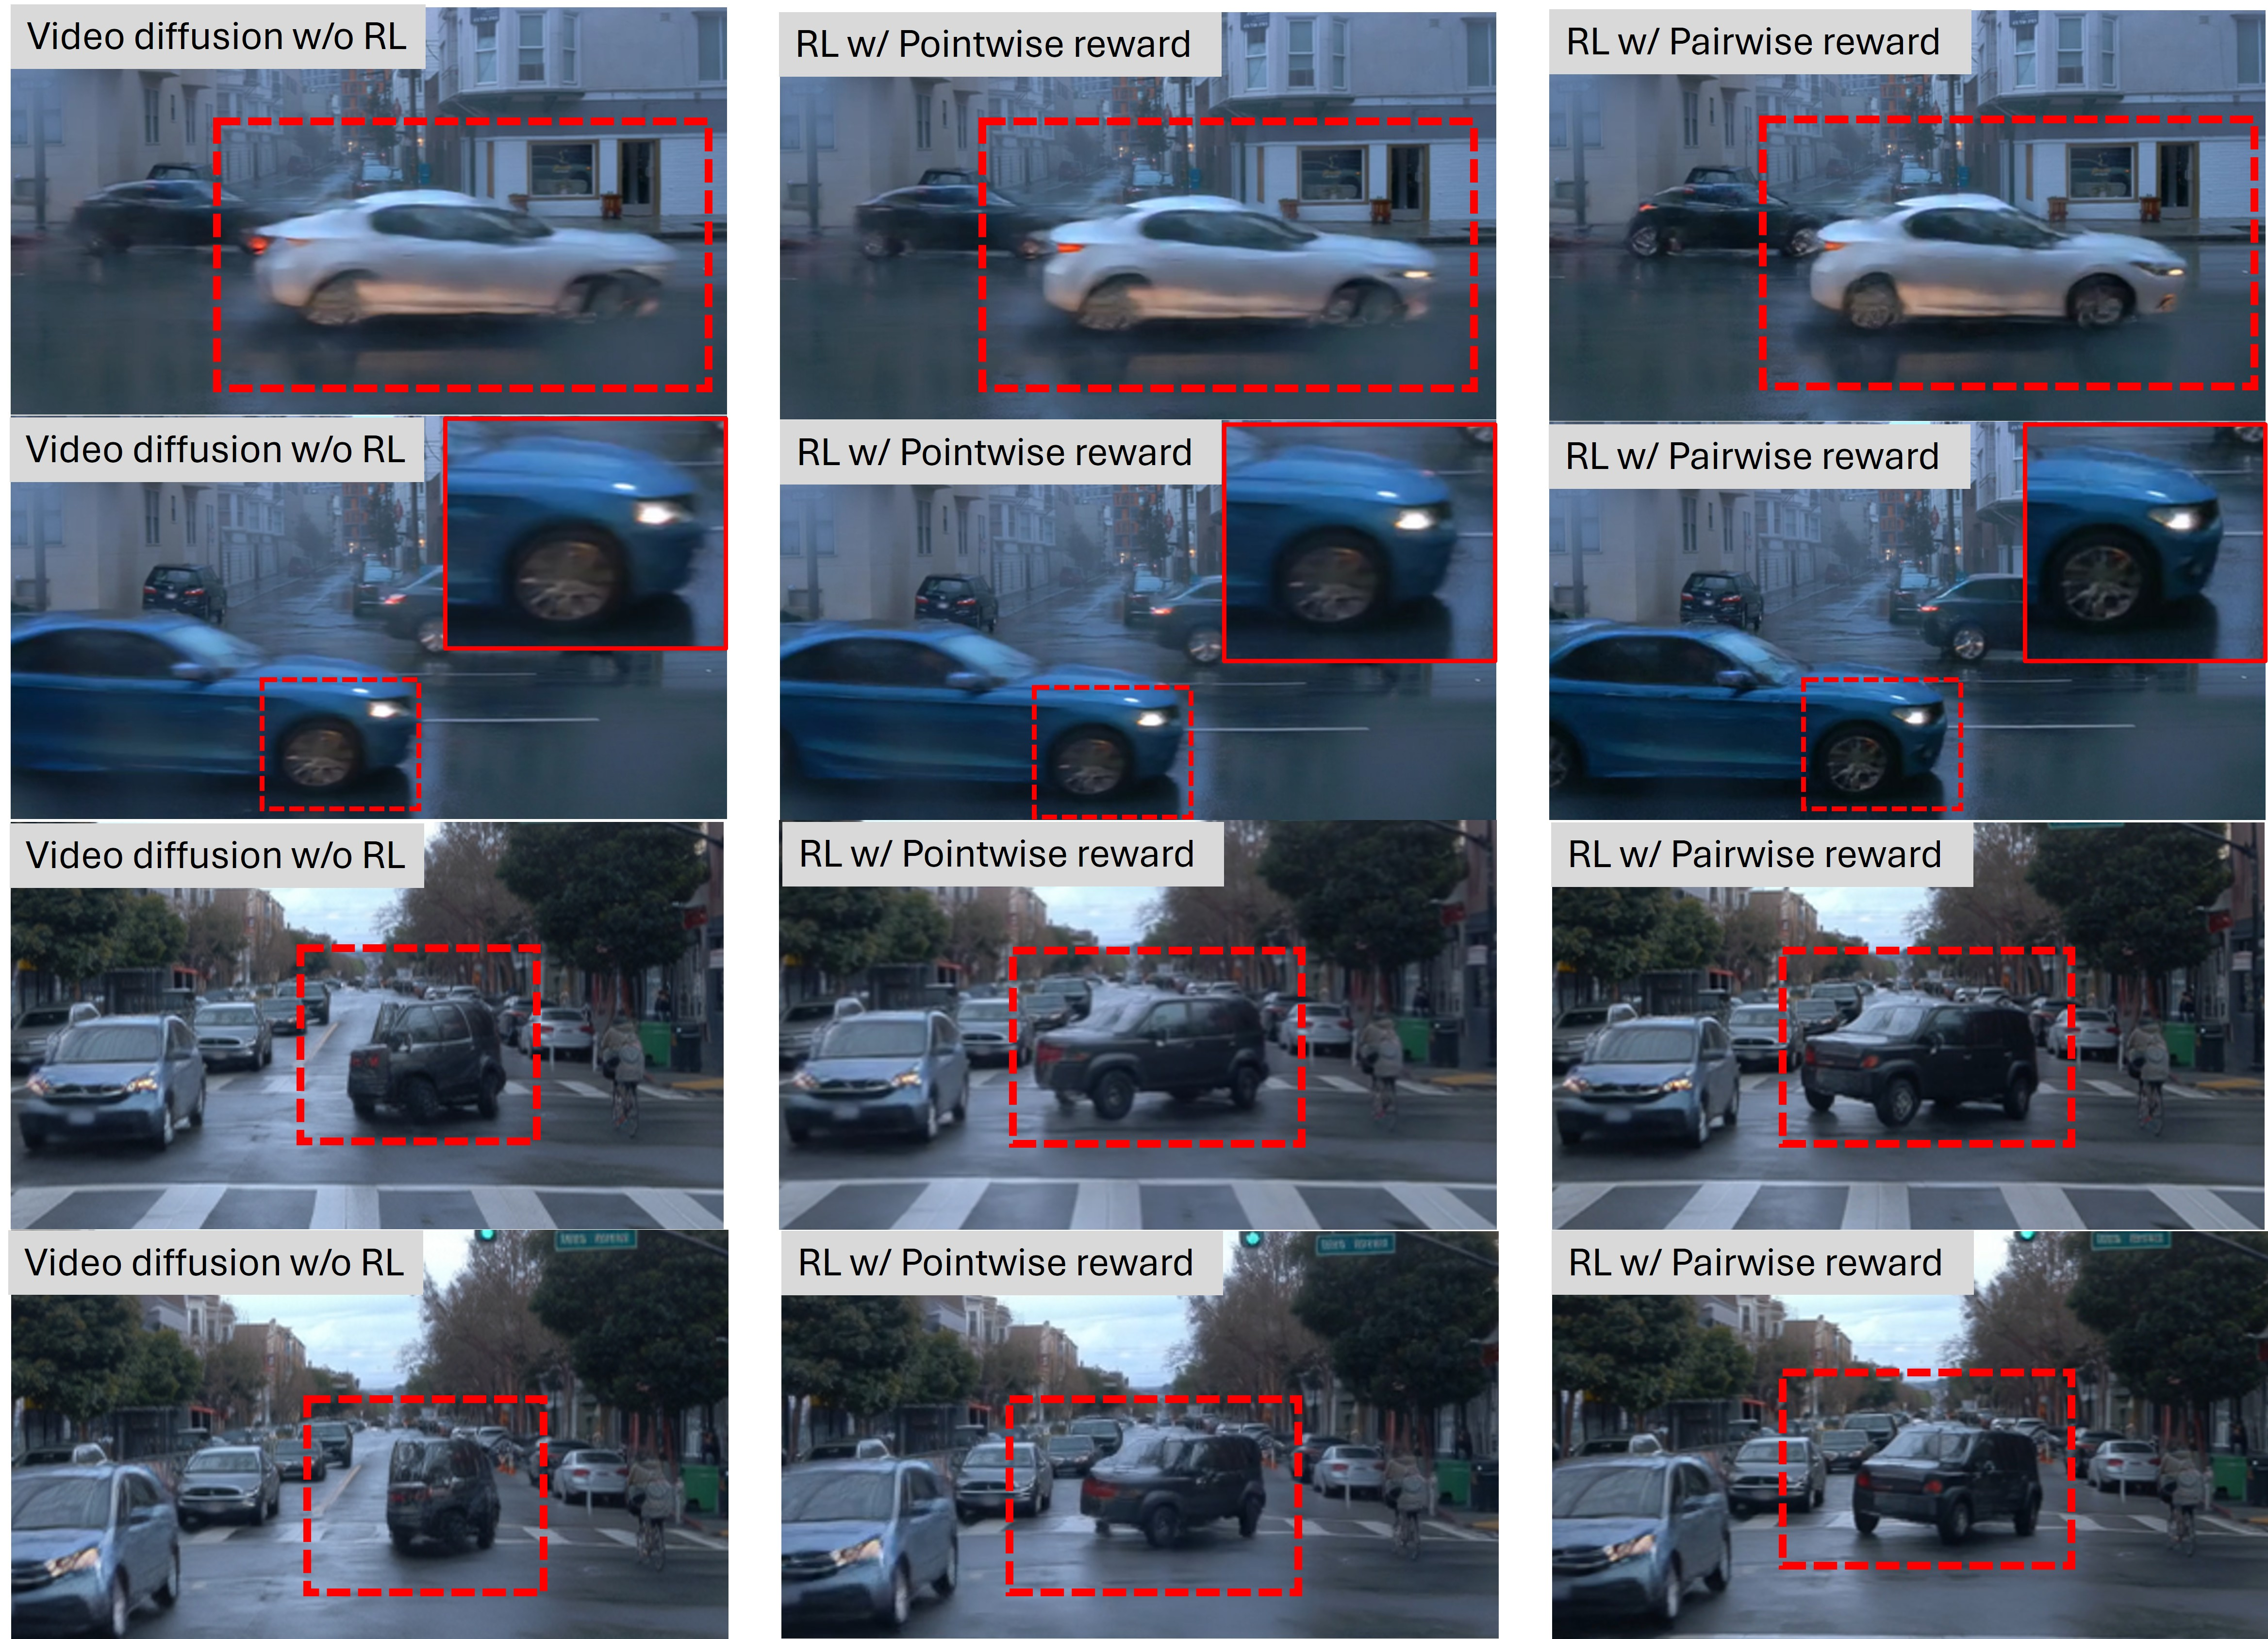
\includegraphics[width=\linewidth]{figures/pointwise_pairwise_comparison.jpg}
    \vspace{-0.2in}
    \caption{\textbf{Qualitative comparison of RL post-training with pointwise vs.\ pairwise reward.} From left to right: video diffusion without RL, RL with pointwise reward, and RL with pairwise reward. Red dashed boxes highlight vehicle regions. While pointwise reward offers limited improvement and sometimes suffers from reward hacking artifacts, the pairwise reward mechanism consistently produces vehicles with better geometry, texture fidelity, and lighting plausibility, demonstrating its superiority as the reward signal for RL post-training.}
    \label{fig:pointwise_pairwise_comparison}
    %\vspace{-0.2in}
    \vspace{-0.2in}
\end{figure}


\subsection{RL post-training comparison.}
We substitute the pairwise reward in our RL pipeline with the pointwise model: each candidate's reward is its independent scalar score $r_i = g(f(I_i))$, with all other settings unchanged. We train both RL with pointwise reward and our method (RL with pairwise reward) on the same 5 OOD scenarios (in-place spinning, left turn, right turn, vehicle rollover, and doubled speed) for 200 steps each. As shown in Fig.\ref{fig:pointwise_pairwise_comparison}, our pairwise reward mechanism produces vehicles with notably better geometry, texture fidelity, and lighting plausibility, especially in the highlighted regions. This corroborates our analysis in Sec.3.2: pointwise scoring is susceptible to reward hacking\cite{Pref-GRPO&UniGenBench}, where negligible absolute score differences are amplified into misleading gradients. In contrast, our pairwise win-rate mechanism aggregates $\binom{N}{2}$ robust comparisons into a discriminative per-candidate reward, providing reliable optimization directions even among similar-quality candidates.


%

\end{document}
